\documentclass[aip,pof,preprint]{revtex4-2}
\usepackage{graphicx}
\usepackage{amsmath}
\usepackage{amssymb}
\usepackage{booktabs}
\usepackage{longtable}
\usepackage{hyperref}
\hypersetup{hidelinks}
\usepackage[utf8]{inputenc}
\usepackage[T1]{fontenc}
\usepackage[english]{babel}

\renewcommand{\figurename}{Figure}
\renewcommand{\tablename}{Table}
\renewcommand{\thefigure}{SM.\arabic{figure}}
\renewcommand{\thetable}{SM.\Roman{table}}

\begin{document}

\title{Supplementary Material for ``Bottom-wall shaping redistributes rather than adds viscous dissipation in a lid-driven cavity: a superelliptic energy-budget analysis''}

\author{Ahmed Beniaiche}
\affiliation{Laboratory of Fluid Mechanics, Ecole Militaire Polytechnique, Algiers, Algeria}

\maketitle

\tableofcontents

\section{Exact geometric definitions and parameter ranges}
\label{suppsec:geometry}

\subsection{Exact geometry}

The bottom boundary of the cavity follows the curve
\begin{equation}
y_b(x)= b\left[1-\left(1-\left|\tfrac{x}{a}\right|^{n}\right)^{1/n}\right]
\;+\;\frac{\alpha}{2}\left[1-\cos\!\left(\frac{2\pi N_w (x+a)}{2a}\right)\right],
\label{suppeq:yb}
\end{equation}
with $a=b=0.5$, $N_w=1$, and $x$ measured from the domain centre. The first term is the superelliptic relief and the second is the single-period undulation. In the lattice implementation the fluid domain is defined by a staircase mask that marks a cell as fluid or solid according to whether its centre lies above or below Eq.~\eqref{suppeq:yb}. This mask only selects the set of active nodes; the hydrodynamic no-slip condition is \emph{not} placed on the staircase interface but on the analytic wall~\eqref{suppeq:yb}, through the Bouzidi interpolated bounce-back described in Section~\ref{suppsec:lbm}: the crossing link is intersected analytically and the fractional distance $q$ to the wall sets the interpolation weights. The relative undulation amplitude is $\alpha=h/L$, where $h$ is the vertical displacement of the boundary and $L$ is the cavity width.

The number of undulations is $N_w=1$ for all cases reported here, so the transitions $n=2\rightarrow4\rightarrow6\rightarrow8$ isolate the effect of the superellipse exponent at fixed undulation count. For $n=2$ the relief is a semicircle of radius $L/2$; as $n$ increases it flattens toward a square bottom with rounded corners.

\subsection{Included configurations}

Table~\ref{supptab:config} lists the parameter ranges and resolutions. The fluid area $A_f$ is not constant across $n$: it increases from $0.8927$ ($n=2$) to $0.9635$ ($n=4$), $0.9819$ ($n=6$), and $0.9892$ ($n=8$) at $\alpha=0$, and from $0.8427$ to $0.9135$, $0.9319$, and $0.9392$ at $\alpha=0.1$. The table gives the ranges of each parameter; it is not a full factorial of the cartesian product, because not every combination was simulated. The cases actually computed are listed case by case in the $N=384$ energetic dataset (Table~\ref{tab:full_scalars384}) and its resolution variants (Table~\ref{supptab:contrasts} and the resolution sweep); no additional cases are implied.

\begin{table}[!htbp]
\centering
\caption{Parameter ranges and resolutions. All cases use the same nominal cavity dimensions; the bottom wall follows Eq.~\eqref{suppeq:yb}. The tabulated values define the ranges explored, not a full cartesian product; only the combinations listed in the energetic dataset were simulated.}
\label{supptab:config}
\begin{tabular}{@{}ll@{}}
\hline
Parameter & Values \\
\hline
Reynolds number, $Re$ & $100$, $400$, $1000$ \\
Superellipse exponent, $n$ & $2$, $4$, $6$, $8$ \\
Relative undulation amplitude, $\alpha$ & $0$, $0.1$ \\
Grid resolution, $N$ & $128$, $256$, $384$ \\
Number of undulations, $N_w$ & $1$ \\
Semi-axes, $a=b$ & $0.5$ \\
Nominal cavity height, $H$ & $1$ \\
Lid velocity, $U_{\mathrm{lid}}$ & $1$ (unit) \\
\hline
Fluid area $A_f$, $\alpha=0$ & $0.8927$, $0.9635$, $0.9819$, $0.9892$ \\
Fluid area $A_f$, $\alpha=0.1$ & $0.8427$, $0.9135$, $0.9319$, $0.9392$ \\
\hline
\end{tabular}
\end{table}

\section{MRT-lattice Boltzmann implementation and numerical parameters}
\label{suppsec:lbm}

\subsection{MRT-LBM details}

The D2Q9 lattice is used with nine discrete velocities. The distribution functions $f_i$ are transformed to moment space via the matrix $\mathbf{M}$, collided with the diagonal relaxation matrix $\mathbf{S}=\mathrm{diag}(s_0,s_1,\dots,s_8)$, and transformed back before streaming. The hydrodynamic moments use relaxation rates $s_0=0$, $s_1=1$, $s_3=s_5=1/\tau$, while the non-hydrodynamic moments are fixed at standard values for stability at low Mach number. The kinematic viscosity is related to the relaxation time by
\begin{equation}
\nu = c_s^2\left(\tau-\tfrac{1}{2}\right)\Delta t, \qquad c_s^2=\tfrac{1}{3}.
\end{equation}
The lattice velocity is set from $U=(\tau-\tfrac12)\,Re/(3N)$, so that $Re=UN/\nu_{\mathrm{lat}}$ with $\nu_{\mathrm{lat}}=\tfrac13(\tau-\tfrac12)$. The lattice Mach number is $Ma=U/c_s$.

\subsection{Lid and curved-wall treatment}

\paragraph{Curved bottom wall.}
The bottom boundary is handled with Bouzidi interpolated bounce-back~\cite{Bouzidi2001}. For each fluid node adjacent to the boundary, the distance $q$ from the node to the wall along the lattice link is measured; the unknown population is reconstructed as a linear interpolation between the wall and the upstream node, weighted by $q$. This second-order treatment resolves the curved boundary without stair-step approximations.

\paragraph{Moving lid.}
The lid velocity is imposed using a regularized momentum injection: the top-wall links receive a prescribed momentum consistent with the lid velocity, smoothed near the corners with a smoothstep profile of width $\varepsilon=0.02$. This is a link-based momentum forcing that reproduces the prescribed lid velocity while mitigating the corner singularity.

\subsection{Parameters by Reynolds number and resolution}

Table~\ref{supptab:params} lists the LBM parameters for each $(Re,N)$ combination used in the primary campaign. The relaxation time $\tau$ is held fixed for each Reynolds number and the lattice velocity follows the diffusive scaling $U=(\tau-\tfrac12)\,Re/(3N)$; as a result $U\propto 1/N$ and the lattice Mach number $Ma = U/c_s$ decreases with refinement. Because $\tau$ is chosen for numerical stability rather than to keep $Ma$ fixed, $Ma$ is not identical across Reynolds numbers: it is largest at the coarsest grid and highest $Re$ ($Ma\approx0.18$ at $N=128$, $Re=400/1000$), and it is $\approx0.06$ or below on the $N=384$ production grid.

\begin{table}[!htbp]
\centering
\caption{Complete numerical parameter set for each Reynolds-number and resolution combination of the primary matrix. Here $\tau$ is fixed per Reynolds number; $U=(\tau-\tfrac12)Re/(3N)$ and $Ma=\sqrt{3}\,U$. Values at $N=384$ are the production grid.}
\label{supptab:params}
\begin{tabular}{@{}ccccc@{}}
\hline
$Re$ & $N$ & $\tau$ & $U$ & $Ma$ \\
\hline
$100$  & $128$ & $0.65$ & $0.039063$ & $0.0677$ \\
$100$  & $256$ & $0.65$ & $0.019531$ & $0.0338$ \\
$100$  & $384$ & $0.65$ & $0.013021$ & $0.0226$ \\
$400$  & $128$ & $0.60$ & $0.104167$ & $0.1804$ \\
$400$  & $256$ & $0.60$ & $0.052083$ & $0.0902$ \\
$400$  & $384$ & $0.60$ & $0.034722$ & $0.0601$ \\
$1000$ & $128$ & $0.54$ & $0.104167$ & $0.1804$ \\
$1000$ & $256$ & $0.54$ & $0.052083$ & $0.0902$ \\
$1000$ & $384$ & $0.54$ & $0.034722$ & $0.0601$ \\
\hline
\end{tabular}
\end{table}

\paragraph{Complete parameter set for the Reynolds sweep.}
To ensure full reproducibility of the continuous Reynolds-number analysis reported in the main text, Table~\ref{supptab:resweep_params} documents the exact LBM parameters for all 19 Reynolds numbers of the $N=128$ fine sweep ($Re=100$ to $1000$ in increments of $50$). At $Re=100$, the run uses $\tau=0.65$ and $U=0.039063$ ($Ma=0.0677$). For all subsequent points $Re\ge150$, the lattice velocity is held constant at $U=5/48\approx0.104167$ ($Ma=\sqrt{3}\,U\approx0.1804$), so that the kinematic viscosity is $\nu_{\rm lat} = 40/(3\,Re)$ and the relaxation time follows the exact relation $\tau = 0.5 + 40/Re$.

\begin{table}[!htbp]
\centering
\caption{Complete LBM numerical parameters for the 19-point exploratory Reynolds-number sweep at $N=128$. For $Re=100$, $\tau=0.65$ and $U=0.039063$ ($Ma=0.0677$). For all $Re\ge150$, the lattice velocity is fixed at $U=5/48\approx0.104167$ ($Ma=\sqrt{3}\,U\approx0.1804$), giving $\nu_{\rm lat} = \frac{40}{3 Re}$ and $\tau = 0.5 + \frac{40}{Re}$.}
\label{supptab:resweep_params}
\begin{tabular}{@{}ccccc|ccccc@{}}
\hline
$Re$ & $\tau$ & $U$ & $Ma$ & $\nu_{\rm lat}$ & $Re$ & $\tau$ & $U$ & $Ma$ & $\nu_{\rm lat}$ \\
\hline
$100$ & $0.65000$ & $0.039063$ & $0.0677$ & $0.050000$ & $550$ & $0.57273$ & $0.104167$ & $0.1804$ & $0.024242$ \\
$150$ & $0.76667$ & $0.104167$ & $0.1804$ & $0.088889$ & $600$ & $0.56667$ & $0.104167$ & $0.1804$ & $0.022222$ \\
$200$ & $0.70000$ & $0.104167$ & $0.1804$ & $0.066667$ & $650$ & $0.56154$ & $0.104167$ & $0.1804$ & $0.020513$ \\
$250$ & $0.66000$ & $0.104167$ & $0.1804$ & $0.053333$ & $700$ & $0.55714$ & $0.104167$ & $0.1804$ & $0.019048$ \\
$300$ & $0.63333$ & $0.104167$ & $0.1804$ & $0.044444$ & $750$ & $0.55333$ & $0.104167$ & $0.1804$ & $0.017778$ \\
$350$ & $0.61429$ & $0.104167$ & $0.1804$ & $0.038095$ & $800$ & $0.55000$ & $0.104167$ & $0.1804$ & $0.016667$ \\
$400$ & $0.60000$ & $0.104167$ & $0.1804$ & $0.033333$ & $850$ & $0.54706$ & $0.104167$ & $0.1804$ & $0.015686$ \\
$450$ & $0.58889$ & $0.104167$ & $0.1804$ & $0.029630$ & $900$ & $0.54444$ & $0.104167$ & $0.1804$ & $0.014815$ \\
$500$ & $0.58000$ & $0.104167$ & $0.1804$ & $0.026667$ & $950$ & $0.54211$ & $0.104167$ & $0.1804$ & $0.014035$ \\
      &           &            &          &            & $1000$ & $0.54000$ & $0.104167$ & $0.1804$ & $0.013333$ \\
\hline
\end{tabular}
\end{table}

\paragraph{Coupled $(\tau,U)$ sensitivity.}
At fixed $Re$ the couple $(\tau,U)$ is not unique: holding $U$ fixed while varying $\tau$ (or vice versa) traces lines of constant $Re$ in the $(Ma,\tau)$ plane. Because $\tau$ enters both the viscosity and, through the Bouzidi $q$-distance, the effective position of the curved wall, we recomputed both states of the primary contrast --- the reference $n=2$ and the flat-bottomed $n=4$ --- at $Re=400$ on two grids and over four lattice speeds $U\in\{0.026042,0.052083,0.104167,0.208333\}$, i.e.\ $Ma\in\{0.045,0.090,0.180,0.361\}$ and, on each grid, $\tau=\tfrac12+3U N/Re$ (Table~\ref{supptab:fitma}).

The energy-balance defect $\varepsilon=(P^*-D^*)/D^*$ (Table~\ref{supptab:fitma}, left) is grid-controlled: at fixed $Ma$ it roughly halves from $N=128$ to $N=256$ (from $-4.24\%$ to $-2.71\%$ at the lowest $Ma$; from $-6.20\%$ to $-3.23\%$ at $Ma=0.18$), the first-order signature of a discretisation error. Its $Ma$ dependence, however, is not negligible on the coarse grid: at $N=128$ the defect moves by $2.0$ percentage points ($-4.24\%$ to $-6.25\%$) over the factor-eight change of $Ma$, whereas at $N=256$ the same range moves it by only $0.6$ point. The coarse-grid $N=128$ Reynolds sweep of the main text therefore carries at least a partial $Ma$ effect, which is why the resolution study is performed at fixed $\tau$ per $Re$ rather than at fixed $Ma$.

What matters for the present work, however, is not the absolute defect but the matched contrast $I_D(2,4)$, which is a difference of the $n=2$ and $n=4$ states computed at the \emph{same} $(\tau,U)$. We computed this contrast at every one of the eight $(N,Ma)$ couples. It varies far less than the defect: at $N=128$ the contrast is $0.32224\%$, $0.32294\%$, $0.32251\%$, and $0.32103\%$ at $Ma=0.045$, $0.090$, $0.180$, and $0.361$, and at $N=256$ it is $0.32465\%$, $0.32462\%$, $0.32407\%$, and $0.32270\%$ (Table~\ref{supptab:fitma}). Across the full factor-eight $Ma$ range, $I_D(2,4)$ changes by only $0.0019$ percentage point on either grid -- a span of about $0.6\%$ of its own value -- whereas the absolute defect moves by $2.0$ points ($N=128$) or $0.6$ point ($N=256$) over the same range. The near-cancellation of the common discretisation and compressibility error in the paired difference is therefore demonstrated, not assumed: the same $Ma$ variation that moves the absolute defect by two points moves the contrast by well under $1\%$ of itself.

\begin{table}[!htbp]
\centering
\caption{Grid$\times$Mach factorial at $Re=400$ for the two states of the primary contrast, $n=2$ (reference) and $n=4$. Because $U$ is held fixed, $\nu=UN/Re$ and $\tau=\tfrac12+3\nu$ depend on the grid; the relaxation time is listed separately for each grid. Columns: lattice speed $U$ and Mach number, relaxation time $\tau$ on each grid, energy-balance defect $\varepsilon=(P^*-D^*)/D^*$ of the reference $n=2$ state (percent), and the matched contrast $I_D(2,4)=100\,(D^*_{4}-D^*_{2})/D^*_{2}$ (percent).}
\label{supptab:fitma}
\begin{tabular}{@{}cccccc@{}}
\hline
$U$ & $Ma$ & $\tau$ ($N{=}128$) & $\tau$ ($N{=}256$) & $\varepsilon$ (\%) & $I_D(2,4)$ (\%) \\
\hline
\multicolumn{6}{@{}l}{$N=128$} \\
$0.026042$ & $0.045$ & $0.525$ & $0.550$ & $-4.238$ & $0.32224$ \\
$0.052083$ & $0.090$ & $0.550$ & $0.600$ & $-5.511$ & $0.32294$ \\
$0.104167$ & $0.180$ & $0.600$ & $0.700$ & $-6.204$ & $0.32251$ \\
$0.208333$ & $0.361$ & $0.700$ & $0.900$ & $-6.253$ & $0.32103$ \\
\multicolumn{6}{@{}l}{$N=256$} \\
$0.026042$ & $0.045$ & $0.525$ & $0.550$ & $-2.709$ & $0.32465$ \\
$0.052083$ & $0.090$ & $0.550$ & $0.600$ & $-3.199$ & $0.32462$ \\
$0.104167$ & $0.180$ & $0.600$ & $0.700$ & $-3.232$ & $0.32407$ \\
$0.208333$ & $0.361$ & $0.700$ & $0.900$ & $-2.611$ & $0.32270$ \\
\hline
\end{tabular}
\end{table}

\section{Iterative convergence and benchmark verification}
\label{suppsec:convergence}

\subsection{Iterative convergence}

Each simulation was run until the relative change of the velocity field between successive measurement windows fell below $10^{-8}$. The final residual and iteration count are recorded for every case in the scalar output files. All $24$ cases at $N=384$ in the main campaign ($N_w=1$, $\alpha\in\{0,0.1\}$) satisfied this criterion, with residuals at or below $9.9\times10^{-9}$ and $478$k--$1.21$M iterations. The convergence history for representative cases is shown in Fig.~\ref{suppfig:residual}.

\begin{figure}[!htbp]
\centering
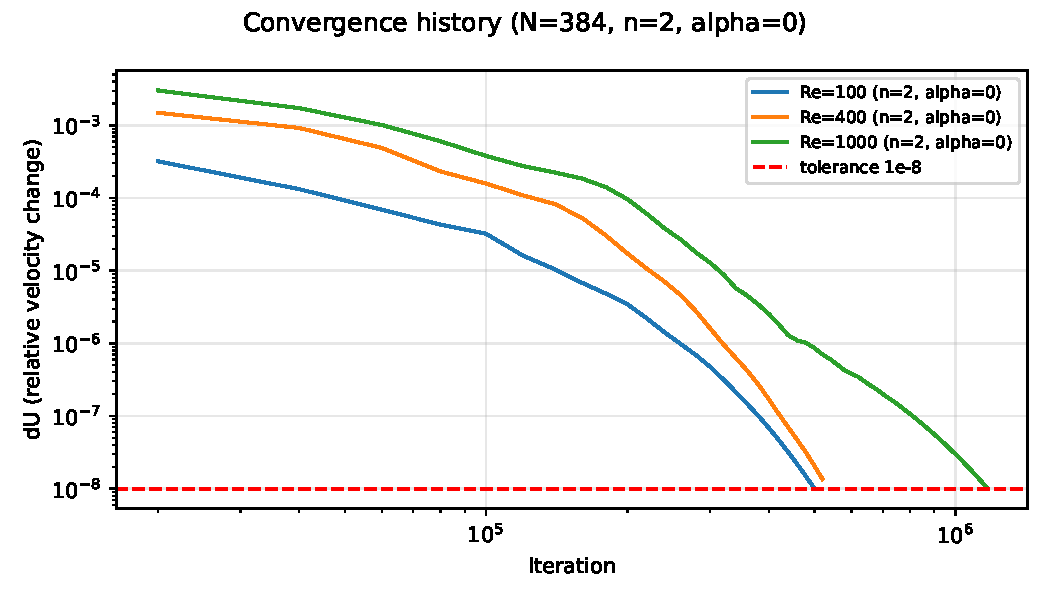
\includegraphics[width=0.8\columnwidth]{figures/figS_residual.pdf}
\caption{Iterative residual versus iteration number for representative cases at $N=384$. All cases converge to residuals at or below $10^{-8}$.}
\label{suppfig:residual}
\end{figure}

\subsection{Benchmark verification against Ghia et al.}

Two distinct comparison cases are reported, to separate the effect of the geometry from that of the lid treatment.

\emph{Exact square cavity.} An exact square cavity with a flat bottom and a \emph{uniform} (non-regularized) lid was run separately at $Re=100$, $400$, and $1000$, and $N=128$--$384$. This isolates the flat-wall and uniform-lid limits of the solver and is the case directly comparable with Ghia et al.~\cite{Ghia1982}. At $N=256$ the maximum absolute centerline deviations are $0.0062$ and $0.0102$ ($Re=100$), $0.0033$ and $0.0058$ ($Re=400$, excluding the single anomalous tabulated datum at $x=0.9063$~\cite{Chai2006}), and $0.0050$ and $0.0136$ ($Re=1000$) for $\max|u-u_G|$ and $\max|v-v_G|$; these reproduce the previously validated reference errors ($0.0057$, $0.0080$, $0.0141$). The exact-square metrics are collected in Table~IV of the main text.

\emph{Near-square campaign case.} The exact square cavity is not one of the campaign geometries; the closest available case is $n=8$, $\alpha=0$, with $A_f=0.9892$ and rounded bottom corners, and it uses the \emph{regularized} lid ($\varepsilon=0.02$) of the production solver. Its centerline profiles were compared with the same benchmark at $N=256$, using the same interior stations and the same exclusion of the anomalous $Re=400$ datum as for the exact square. The maximum absolute deviations are $0.0038$ and $0.0054$ ($Re=100$), $0.0035$ and $0.0034$ ($Re=400$), and $0.0046$ and $0.0066$ ($Re=1000$) for $\max|u-u_G|$ and $\max|v-v_G|$---of the same order as, and in several cases smaller than, the exact-square values. The curved-wall (Bouzidi) treatment and the near-square bottom therefore do not degrade the interior solution despite the regularized lid, which differs from the uniform lid of Ghia at the top corners. Neither comparison validates the energetic integrals, whose grid sensitivity is treated in Section~\ref{suppsec:consistency}. Detailed metrics are given in Table~\ref{supptab:benchmark}.

\begin{table}[!htbp]
\centering
\caption{Benchmark verification against Ghia et al.~\cite{Ghia1982}. Top block: exact square cavity (flat bottom, uniform lid), maximum absolute deviations $\max|u-u_G|$ ($x=0.5$) and $\max|v-v_G|$ ($y=0.5$) at $N=256$; the single anomalous tabulated datum at $(Re{=}400,\,x{=}0.9063)$~\cite{Chai2006} is excluded from $\max|v-v_G|$ in the final column. Bottom block: near-square campaign case $n=8$, $\alpha=0$ ($A_f=0.9892$, regularized lid), same interior stations and same exclusion.}
\label{supptab:benchmark}
\begin{tabular}{@{}lcccc@{}}
\hline
Case & $Re$ & $\max|u-u_G|$ & $\max|v-v_G|$ & excl. \\
\hline
exact square & $100$  & $0.0062$ & $0.0102$ & $0.0102$ \\
exact square & $400$  & $0.0033$ & $0.1492$ & $0.0058$ \\
exact square & $1000$ & $0.0050$ & $0.0136$ & $0.0136$ \\
\hline
$n=8$, $\alpha=0$ & $100$  & $0.0038$ & $0.0054$ & $0.0054$ \\
$n=8$, $\alpha=0$ & $400$  & $0.0035$ & $0.1425$ & $0.0034$ \\
$n=8$, $\alpha=0$ & $1000$ & $0.0046$ & $0.0141$ & $0.0066$ \\
\hline
\end{tabular}
\end{table}

\begin{table}[!htbp]
\centering
\caption{Isolating the effect of the regularized production lid on a \emph{strictly flat} square cavity ($A_f=1$). The complete $Re\times N\times$lid matrix is reported as the maximum interior-centerline deviations from Ghia et al.~\cite{Ghia1982} ($\max|u-u_G|$ / $\max|v-v_G|$), using the same interior stations and the same exclusion of the anomalous $Re=400$ datum at $x=0.9063$. The last two columns give the regularized-minus-uniform change; it never exceeds $5.5\times10^{-4}$. The lid regularization therefore removes only the corner singularity and does not measurably bias the interior flow.}
\label{supptab:lidreg}
\begin{tabular}{@{}lccc@{}}
\hline
$Re$ & $N$ & $\max|u-u_G|$ / $\max|v-v_G|$ (uniform) & $\max|u-u_G|$ / $\max|v-v_G|$ (regularized) \\
\hline
100  & 128 & $0.00754$ / $0.01091$ & $0.00752$ / $0.01092$ \\
100  & 256 & $0.00623$ / $0.01020$ & $0.00622$ / $0.01019$ \\
400  & 128 & $0.00800$ / $0.00746$ & $0.00810$ / $0.00755$ \\
400  & 256 & $0.00329$ / $0.00580$ & $0.00334$ / $0.00578$ \\
1000 & 128 & $0.01197$ / $0.01069$ & $0.01251$ / $0.01119$ \\
1000 & 256 & $0.00502$ / $0.01358$ & $0.00516$ / $0.01347$ \\
\hline
\end{tabular}
\end{table}

\subsection{Independent-solver cross-validation}
\label{suppsec:crosscheck}

As a final check that the energetic contrasts are not an artifact of the MRT-LBM discretisation, the two-member primary contrast $I_D(2,4)$ at $Re=400$, $\alpha=0$ was recomputed with a completely independent solver: a conforming Taylor--Hood finite-element method (P2 velocity / P1 pressure, Picard linearisation) on a boundary-fitted mesh graded toward the wall and the lid. The geometry function was replaced by the superelliptic wall of Eq.~\eqref{suppeq:yb} so that both solvers integrate over the identical domain, and the same regularized lid profile is imposed in both: the finite-element solver prescribes the identical cubic-smoothstep lid velocity $U(x)=U_{\rm lid}\,g(x)$ with the same corner-regularization width $\varepsilon=0.02$ used by the lattice-Boltzmann production run (a prescribed Dirichlet velocity on the top boundary for the FEM, the corresponding regularized momentum injection for the LBM). All finite-element energetics are reported \emph{natively}: the strain-rate, lid-power, and kinetic-energy integrals are evaluated element-wise from the finite-element velocity field, with no projection onto the LBM grid and no LBM wall-gradient model. The native finite-element energy balance closes to $0.01\%$ at the finest mesh ($P^*=D^*$ to $0.01\%$), and within $0.22\%$ over all meshes (Table~\ref{supptab:femconv}). The meshes $nx=ny=64,128,256$ were run for both $n=2$ and $n=4$.

The independent finite-element calculations provide a cross-solver consistency check. At the finest available resolutions the finite-element and lattice-Boltzmann dissipation contrasts differ by approximately $0.002$ percentage points ($I_D(2,4)=+0.323\%$ at $nx=256$ versus $+0.325\%$ at $N=384$). The finite-element estimates, however, span $0.023$ percentage points across the three meshes ($+0.346\%$, $+0.332\%$, $+0.323\%$ at $nx=64,128,256$), which exceeds the finest-grid FEM--LBM gap; this agreement is therefore not interpreted as evidence of finite-element convergence toward the lattice-Boltzmann value (Table~\ref{supptab:crosscheck}). The FEM calculation is reported throughout strictly as a cross-solver consistency check, at $Re=400$ and (Section below) at $Re=1000$, and never as a convergence result for either solver. On the matched finest grids (FEM $nx=256$, LBM $N=384$) the absolute levels agree to a few percent ($K^*: +1.1\%$, $D^*: +2.0\%$, $P^*: +4.1\%$), and all three contrasts agree to within $0.02$ percentage point ($I_K: 0.019$~pt, $I_P: 0.008$~pt, $I_D: 0.002$~pt). The larger $P^*$ offset combines the coarser resolution of the lid shear layer at $N=384$ with the residual $2\%$ lattice-Boltzmann power--dissipation imbalance at that grid; both are grid effects that cancel in the paired contrast, exactly as the main text argues.

\emph{Cross-check at $Re=1000$.} The two coarser meshes were also run at $Re=1000$, where the primary contrast is an order of magnitude larger than at $Re=400$. The native finite-element contrast is $+0.716\%$ at $nx=64$ and $+0.598\%$ at $nx=128$, against $+0.5909\%$ at $N=384$ in the lattice-Boltzmann production set: the finer mesh differs by $0.008$ percentage point, or $1.3\%$ in relative terms, and the sequence moves toward the lattice-Boltzmann value under refinement. The native energy balance of these runs closes to $+0.41\%$ ($n=2$) and $+0.21\%$ ($n=4$) at $nx=64$ and to $+0.16\%$ and $+0.15\%$ at $nx=128$. The $nx=256$ mesh was not attempted at $Re=1000$: a single case commits about $9$~GB for the sparse assembly, which cannot be accommodated on this node while the lattice-Boltzmann campaigns are running. The finite-element variation across its own two meshes at this Reynolds number ($0.117$ percentage point) again exceeds the finest-grid finite-element--lattice-Boltzmann gap ($0.008$ percentage point), so this second comparison is reported with the same restriction as at $Re=400$: it is a cross-solver consistency check, not an independent convergence proof for either solver.

\begin{table}[!htbp]
\centering
\caption{Independent-solver cross-validation at $Re=400$ and $Re=1000$, $\alpha=0$: Taylor--Hood FEM (native, $nx=ny=64/128/256$) versus the MRT-LBM ($N=128/256/384$). Top: mesh sensitivity of the native finite-element dissipation contrast $I_D(2,4)$ at both Reynolds numbers; the $nx=256$ finite-element mesh was not run at $Re=1000$, where the memory cost of the sparse assembly exceeds the budget available during the lattice-Boltzmann campaigns. Bottom: absolute $n=2$ reference values and the geometric contrasts, on the finest grids of each solver (FEM $nx=256$, LBM $N=384$). All finite-element entries are native (element-wise integrals, no projection); the LBM-grid-projected finite-element contrasts are $+6.1\%$ ($Re=400$, $nx=64$), $+2.0\%$ ($Re=400$, finest native mesh), $+32.6\%$ and $+11.8\%$ ($Re=1000$, $nx=64$ and $128$), and are not used in any comparison.}
\label{supptab:crosscheck}
\begin{tabular}{@{}lcccc@{}}
\hline
$nx$ & $64$ & $128$ & $256$ & LBM $N=384$ \\
\hline
$I_D(2,4)$ [\%], $Re=400$  & $+0.346$ & $+0.332$ & $+0.323$ & $+0.325$ \\
$I_D(2,4)$ [\%], $Re=1000$ & $+0.716$ & $+0.598$ & --- & $+0.591$ \\
\hline
\end{tabular}

\vspace{4pt}

\begin{tabular}{@{}lccc@{}}
\hline
Quantity (finest grids) & FEM ($nx=256$) & LBM ($N=384$) & rel.\ diff. \\
\hline
$K^*$ ($n=2$), native   & $0.040440$ & $0.040011$ & $+1.1\%$ \\
$P^*$ ($n=2$), native   & $23.899$   & $22.954$   & $+4.1\%$ \\
$D^*$ ($n=2$), native   & $23.896$   & $23.432$   & $+2.0\%$ \\
\hline
$I_K(2,4)$              & $+0.752\%$ & $+0.771\%$ & $0.019$~pt \\
$I_P(2,4)$              & $+0.321\%$ & $+0.328\%$ & $0.008$~pt \\
$I_D(2,4)$              & $+0.323\%$ & $+0.325\%$ & $0.002$~pt \\
\hline
\end{tabular}
\end{table}

\begin{table}[!htbp]
\centering
\caption{Native finite-element mesh-refinement study at $Re=400$, $\alpha=0$: absolute $n=2$ and $n=4$ values of $K^*$, $P^*$, $D^*$ and the native energy balance $P^*/D^*-1$, together with the exact mesh fluid area against the analytic superellipse area ($A_f=0.892699$ for $n=2$, $0.963519$ for $n=4$). The balance stays within $0.22\%$ at all meshes and reaches $0.01\%$ on the finest mesh, and the mesh fluid area approaches the analytic superellipse area under refinement.}
\label{supptab:femconv}
\begin{tabular}{@{}lcccccc@{}}
\hline
$n$ & $nx$ & $K^*$ & $P^*$ & $D^*$ & $P^*/D^*-1$ & $A_f^{\mathrm{mesh}}$ \\
\hline
2 & 64  & $0.040420$ & $23.804$ & $23.819$ & $-0.06\%$ & $0.891888$ \\
2 & 128 & $0.040434$ & $23.960$ & $23.908$ & $+0.22\%$ & $0.892412$ \\
2 & 256 & $0.040440$ & $23.899$ & $23.896$ & $+0.01\%$ & $0.892598$ \\
4 & 64  & $0.040702$ & $23.872$ & $23.901$ & $-0.12\%$ & $0.960547$ \\
4 & 128 & $0.040729$ & $24.038$ & $23.987$ & $+0.21\%$ & $0.962268$ \\
4 & 256 & $0.040744$ & $23.975$ & $23.973$ & $+0.01\%$ & $0.962993$ \\
\hline
\end{tabular}
\end{table}

\section{Additional flow fields and vortex diagnostics}
\label{suppsec:fields}

\subsection{Additional fields}

Figures~\ref{suppfig:fields_alpha0} and~\ref{suppfig:fields_alpha01} collect all twenty-four converged configurations at $N=384$, split by amplitude: $\alpha=0$ and $\alpha=0.1$, respectively. Presenting the two amplitudes in separate figures ensures that undulated and non-undulated cases are never superposed for the same geometry. In each figure the rows correspond to $Re=100$, $400$, and $1000$ and the columns to the full exponent sequence $n=2,4,6,8$, so that every panel is filled. The main manuscript (Fig.~3) shows the $Re=400$ row of both amplitudes at a larger panel size; the present figures extend that selection to the two remaining Reynolds numbers without mixing amplitudes. Within each figure all panels share one colour scale, set by the largest velocity magnitude over its twelve configurations.

\begin{figure}[!htbp]
\centering
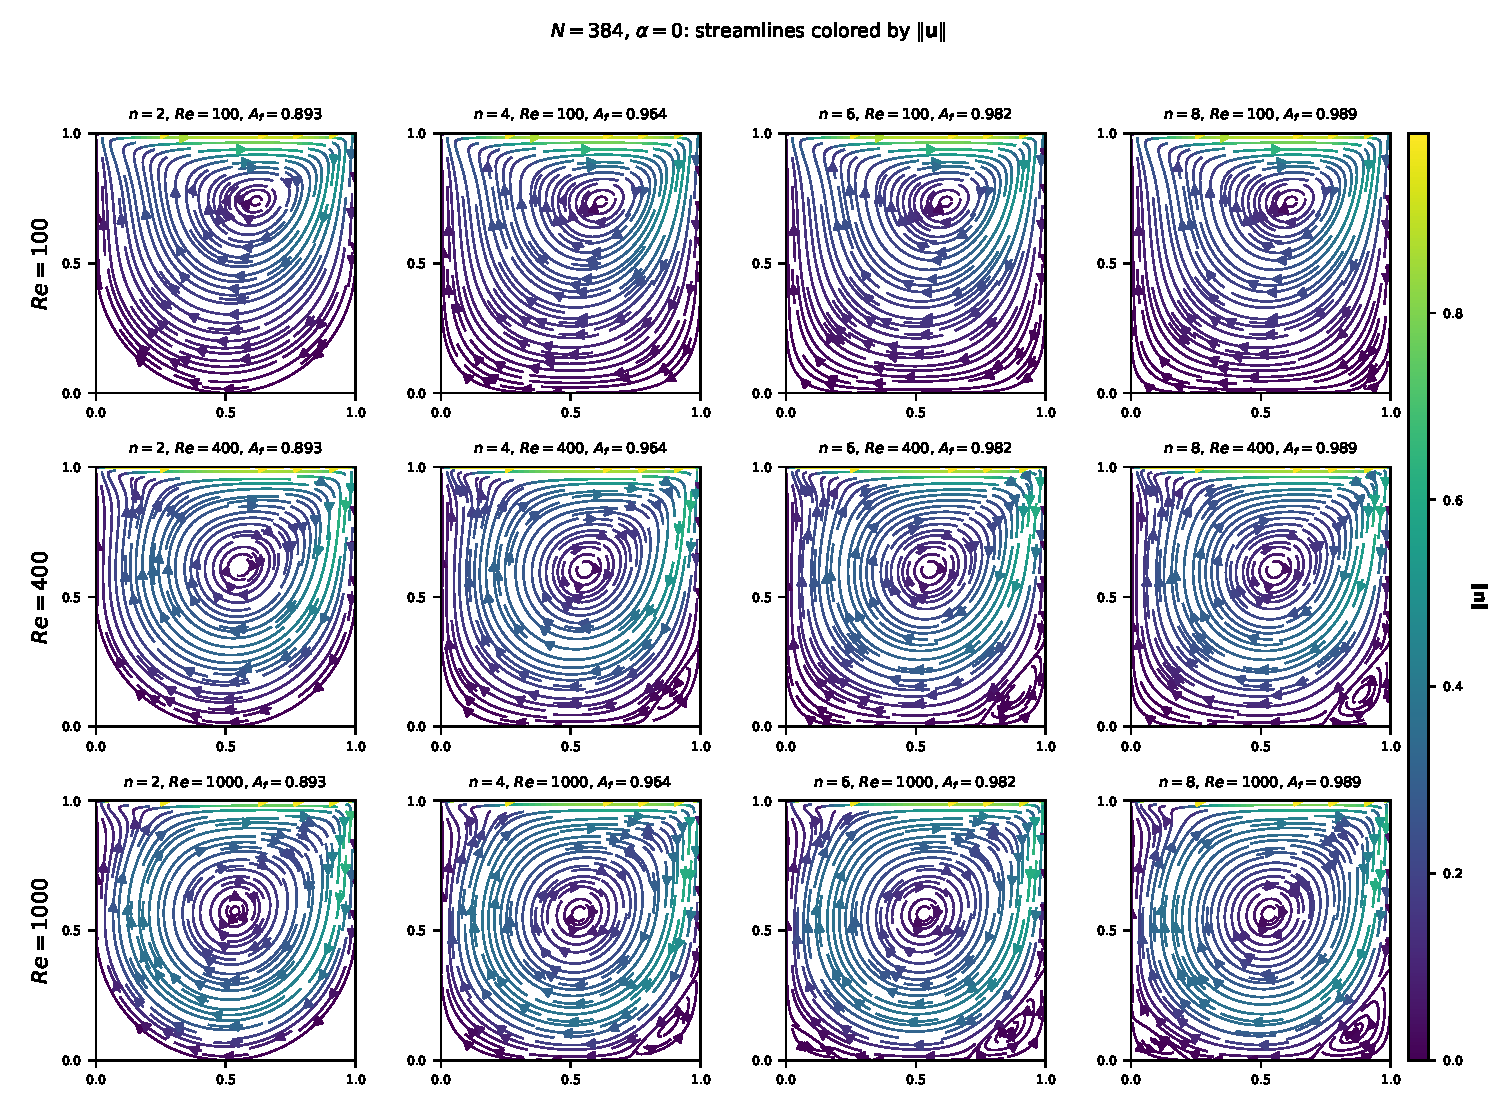
\includegraphics[width=0.95\columnwidth]{figures/figS_fields_alpha0.pdf}
\caption{Streamlines colored by velocity magnitude for the twelve converged $\alpha=0$ configurations at $N=384$. Rows: $Re=100$, $400$, $1000$; columns: $n=2$, $4$, $6$, $8$. Each panel is labeled with its exponent, Reynolds number and fluid area $A_f$, and the color scale is common to all panels of the figure.}
\label{suppfig:fields_alpha0}
\end{figure}

\begin{figure}[!htbp]
\centering
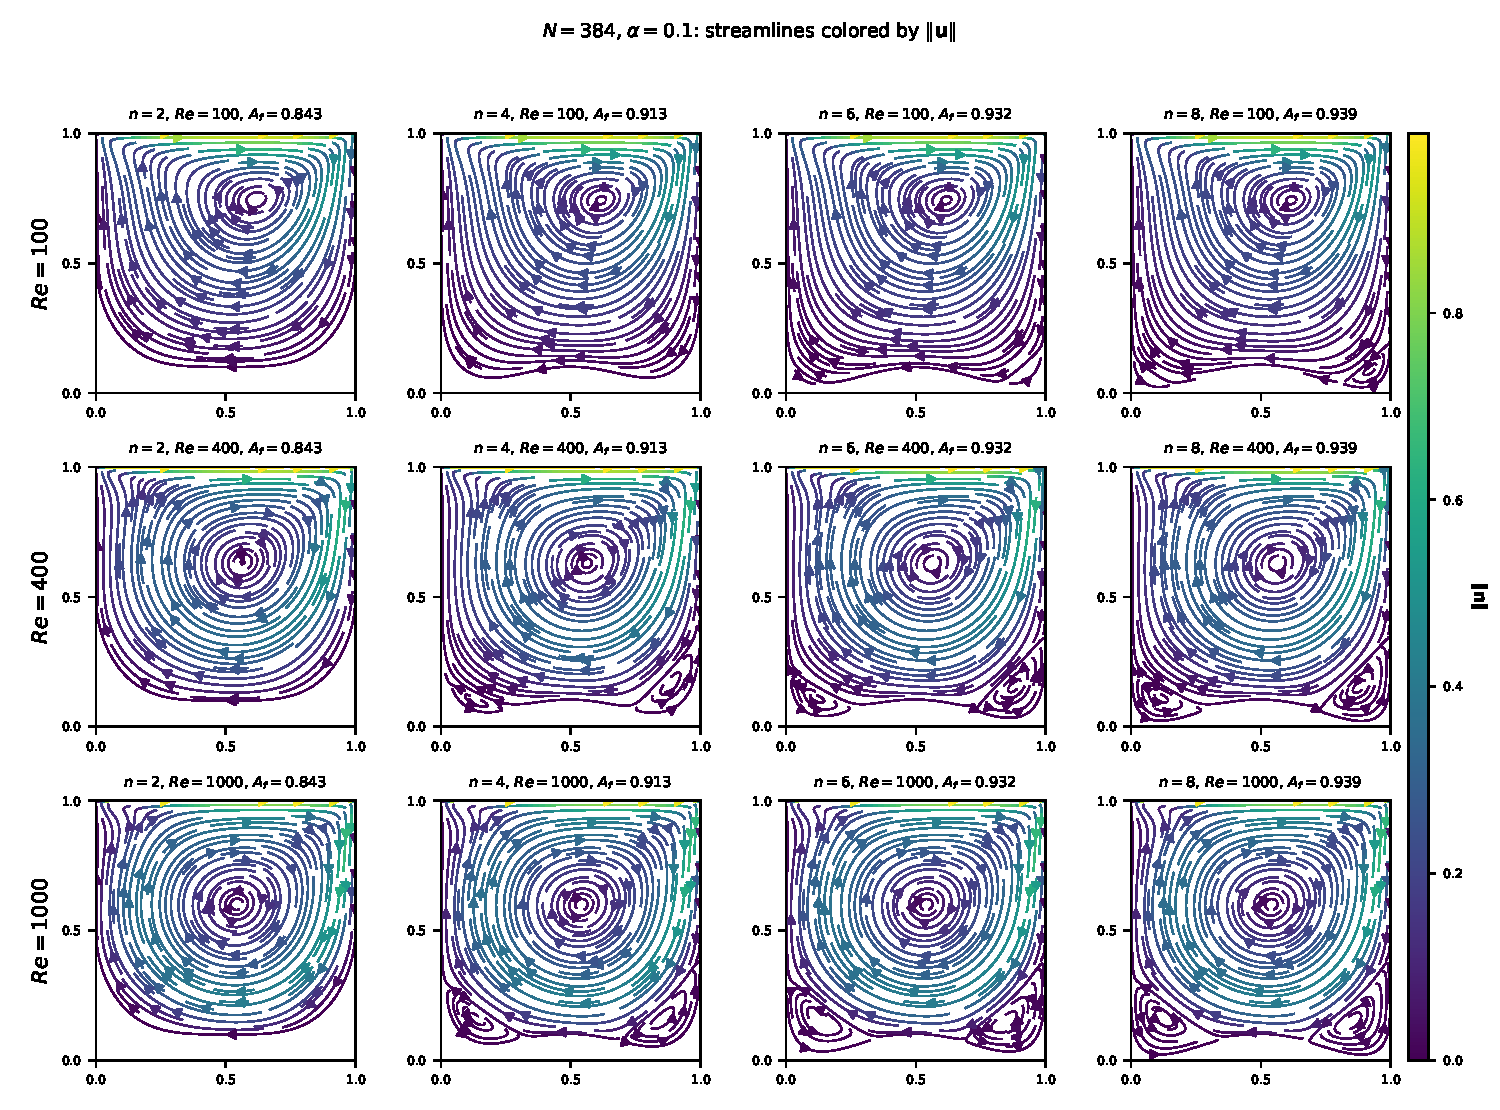
\includegraphics[width=0.95\columnwidth]{figures/figS_fields_alpha01.pdf}
\caption{Same as Fig.~\ref{suppfig:fields_alpha0} for $\alpha=0.1$. The undulated cases are kept separate from the non-undulated fields of Fig.~\ref{suppfig:fields_alpha0}; the wavy bottom wall and the corner vortices it nucleates at $Re\ge400$ are visible in every column.}
\label{suppfig:fields_alpha01}
\end{figure}

\subsection{Vortex diagnostics}

Vortex locations and counts were extracted from the converged fields using a simple critical-point detection: the velocity gradient tensor is evaluated at each grid point, and points where both velocity components vanish (within a tolerance) are classified as centers or saddles. The primary vortex is identified as the center with the largest circulation. This diagnostic is used qualitatively in the main text; a complete vortex census is not included because the energetic contrasts are the primary focus of the analysis.

\section{Complete energetic dataset}
\label{suppsec:energetics}

\subsection{Absolute values}

Table~\ref{tab:full_scalars384} provides the complete energetic dataset for all $24$ cases at $N=384$ in the main campaign ($N_w=1$, $\alpha\in\{0,0.1\}$).

\begin{table}[!htbp]
\centering
\caption{Complete energetic dataset at $N=384$ for all simulated configurations.}
\label{tab:full_scalars384}
\begin{tabular}{@{}ccccccc@{}}
\hline
$Re$ & $n$ & $\alpha$ & $P^*$ & $D^*$ & $K^*$ & $A_f$ \\
\hline
100 & 2 & 0.00 & 17.5612 & 17.9152 & 0.03404 & 0.89271 \\
100 & 2 & 0.10 & 17.5589 & 17.9129 & 0.03368 & 0.84280 \\
100 & 4 & 0.00 & 17.5649 & 17.9191 & 0.03427 & 0.96356 \\
100 & 4 & 0.10 & 17.5602 & 17.9144 & 0.03382 & 0.91349 \\
100 & 6 & 0.00 & 17.5654 & 17.9196 & 0.03428 & 0.98206 \\
100 & 6 & 0.10 & 17.5603 & 17.9145 & 0.03382 & 0.93197 \\
100 & 8 & 0.00 & 17.5654 & 17.9197 & 0.03428 & 0.98934 \\
100 & 8 & 0.10 & 17.5603 & 17.9145 & 0.03382 & 0.93932 \\
400 & 2 & 0.00 & 22.9535 & 23.4318 & 0.04001 & 0.89271 \\
400 & 2 & 0.10 & 22.8349 & 23.3131 & 0.03932 & 0.84280 \\
400 & 4 & 0.00 & 23.0289 & 23.5080 & 0.04032 & 0.96356 \\
400 & 4 & 0.10 & 22.8654 & 23.3442 & 0.03947 & 0.91349 \\
400 & 6 & 0.00 & 23.0315 & 23.5110 & 0.04033 & 0.98206 \\
400 & 6 & 0.10 & 22.8644 & 23.3433 & 0.03949 & 0.93197 \\
400 & 8 & 0.00 & 23.0315 & 23.5110 & 0.04034 & 0.98934 \\
400 & 8 & 0.10 & 22.8640 & 23.3429 & 0.03949 & 0.93932 \\
1000 & 2 & 0.00 & 30.8688 & 31.5439 & 0.04334 & 0.89271 \\
1000 & 2 & 0.10 & 30.5220 & 31.1982 & 0.04248 & 0.84280 \\
1000 & 4 & 0.00 & 31.0547 & 31.7303 & 0.04357 & 0.96356 \\
1000 & 4 & 0.10 & 30.5463 & 31.2226 & 0.04267 & 0.91349 \\
1000 & 6 & 0.00 & 31.0566 & 31.7336 & 0.04361 & 0.98206 \\
1000 & 6 & 0.10 & 30.5385 & 31.2150 & 0.04272 & 0.93197 \\
1000 & 8 & 0.00 & 31.0553 & 31.7324 & 0.04362 & 0.98934 \\
1000 & 8 & 0.10 & 30.5368 & 31.2134 & 0.04274 & 0.93932 \\
\hline
\end{tabular}
\end{table}


\subsection{Fluid areas and normalized quantities}

The fluid area increases with $n$ at fixed $\alpha$: $A_f=0.89271$, $0.96356$, $0.98206$, and $0.98934$ for $n=2,4,6,8$ at $\alpha=0$, and $A_f=0.84280$, $0.91349$, $0.93197$, and $0.93932$ for $n=2,4,6,8$ at $\alpha=0.1$. The area-normalized dissipation is defined as $\overline{D}_A^* = D^*/A_f$. Because $A_f$ changes with $n$, the area-normalized contrast across $n$ differs from the un-normalized contrast; this difference is the content of the area-reference analysis of Section~\ref{suppsec:area}.


\section{Pairwise contrast audit}
\label{suppsec:contrasts}

\subsection{Recomputation of the contrasts}

The matched contrasts are computed directly from the absolute scalar values:
\begin{equation}
I_D(q_i,q_j) = \frac{D^*(q_j)-D^*(q_i)}{D^*(q_i)}\times 100\%, \qquad
I_P(q_i,q_j) = \frac{P^*(q_j)-P^*(q_i)}{P^*(q_i)}\times 100\%.
\end{equation}
The sign convention is fixed: a positive $I_D$ indicates that the higher-exponent geometry dissipates more energy than the lower-exponent one, relative to the latter.

\subsection{Sign and normalization conventions}

The denominator in the percentage is always $D^*(q_i)$ (or $P^*(q_i)$) of the earlier configuration in the pair. The three transitions studied are $(2,4)$, $(4,6)$, and $(6,8)$; the full sequence is available at all three Reynolds numbers. The full contrast dataset for all resolutions is provided in Table~\ref{supptab:contrasts}, which also lists, for every transition and amplitude, the span of $I_D$ over $N=128$, $256$, $384$, and $512$ (the last resolution available only at $Re=400$ and $Re=1000$, $\alpha=0$). That span is the resolution floor of the contrast itself, and the working criterion throughout is that a contrast is resolved only when $|I_D|$ at the finest available resolution exceeds it.

At $Re=400$ the $(6,8)$ contrast at $\alpha=0$ is $+6\times 10^{-5}\%$ against a floor of $1.1\times 10^{-4}$ percentage points, so it is reported only as an upper bound and its sign is not stable across grids. The same transition at $\alpha=0.1$ ($-0.0017\%$, floor $8.5\times 10^{-5}$) and the $(4,6)$ contrast at both amplitudes ($+0.0129\%$, floor $5.0\times 10^{-4}$, and $-0.0039\%$, floor $8.7\times 10^{-4}$) are resolved, the spans being $5\%$, $3.9\%$ and $23\%$ of their magnitudes. At $Re=1000$ both trailing transitions are resolved: $(4,6)=+0.0103\%$ and $(6,8)=-0.0037\%$ at $\alpha=0$, with spans over $N=128$--$512$ of $6.9\times10^{-4}$ and $1.1\times10^{-4}$ percentage points, and $(4,6)=-0.0242\%$, $(6,8)=-0.0052\%$ at $\alpha=0.1$, with spans of $2.2\times10^{-3}$ and $5.5\times10^{-4}$ percentage points. At the undulated wall the two trailing transitions are already negative at $Re=400$ ($-0.0039\%$ and $-0.0017\%$), each larger in magnitude than its own span. The $N=512$ data at $Re=1000$ confirm the monotonicity of the $(2,4)$ contrast ($+0.592\%$) and strengthen the negative sign of the $(6,8)$ transition ($-0.0036\%$).

At $Re=100$ the trailing transitions are $+0.00296\%$ and $+0.00042\%$ at $\alpha=0$, and $+0.00098\%$ and $+0.00006\%$ at $\alpha=0.1$. Only part of this set is directly usable. On the two coarser grids the $n\ge 6$ cases at this Reynolds number run at $Ma_{\max}=0.18$ and $0.09$ while their $n=4$ partners run at $0.068$ and $0.034$, so the coarse members of the $(4,6)$ sequence are not in the same compressibility regime as the reference; the $1.145$ percentage-point apparent span therefore measures that mismatch rather than grid convergence, and no resolution floor can be assigned to the $Re=100$ $(4,6)$ contrast, whose $N=384$ value is quoted as an upper bound. The $(6,8)$ pairs match in Mach number on every grid, their compressibility error cancels in common mode, and their spans ($8.1\times 10^{-5}$ and $5.5\times 10^{-5}$ percentage points) are genuine floors: $+0.00042\%$ at $\alpha=0$ is resolved at $5.2$ times its span, while $+0.00006\%$ at $\alpha=0.1$ is marginal at $1.1$ times its span and is quoted for completeness only.

\begin{table}[!htbp]
\footnotesize
\centering
\renewcommand{\arraystretch}{0.92}
\setlength{\tabcolsep}{3.5pt}
\caption{Full contrast dataset for all resolutions, transitions and amplitudes. $\delta_{IP/ID}=100|I_P/I_D-1|$ is the relative estimator discrepancy and the second-to-last column is the absolute power-minus-dissipation contrast difference, both in percentage points (pp). The last column, printed once per transition and amplitude on its $N=384$ row, is the \emph{own resolution span} of that contrast: the range of $I_D$ over $N=128$, $256$, $384$, and $512$ (the last resolution available only at $Re=400$ and $Re=1000$, $\alpha=0$). A contrast is treated as resolution-resolved only when $|I_D|$ at the finest available resolution exceeds its own span; by that criterion every $(2,4)$ contrast at $\alpha=0$, the trailing $(4,6)$ and $(6,8)$ contrasts at $Re=1000$ for both amplitudes, $(4,6)$ at $Re=400$ and $\alpha=0$, and $(6,8)$ at $Re=400$ and $\alpha=0.1$ are resolved, whereas $Re=400$, $(6,8)$, $\alpha=0$ ($0.00006\%$ against a $0.00011$~pp span) is not and is quoted only as an upper bound. The $Re=100$ trailing spans require a separate caveat: at $N=128$ and $256$ the $n\ge6$ cases sit at local Mach number $Ma_{\max}\simeq 0.18$ and $0.09$ while the $n=4$ reference is at $0.068$ and $0.034$, so the $(4,6)$ pairs compare different compressibility regimes and their spans ($1.145$~pp) measure that mismatch rather than grid convergence. The $(6,8)$ pairs match in Mach number at every $N$, their errors cancel in common mode, and their spans ($8\times10^{-5}$ and $5\times10^{-5}$~pp) are genuine resolution floors; the $Re=100$, $(4,6)$ values at $N=384$ are accordingly quoted as upper bounds. Entries with $|I_D|<10^{-4}\%$ have a numerically meaningless $\delta_{IP/ID}$ and are marked ``--''.}
\label{supptab:contrasts}
\begin{tabular}{@{}ccccccccc@{}}
\hline
$Re$ & $N$ & Transition & $\alpha$ & $I_D$ [\%] & $I_P$ [\%] & $\delta_{IP/ID}$ [\%] & $I_P-I_D$ [pp] & span [pp] \\
\hline
100  & 128 & $(2,4)$ & 0.00 & $+0.02161$ & $+0.01971$ &  8.77 & $-0.00189$ &  \\
100  & 256 & $(2,4)$ & 0.00 & $+0.02195$ & $+0.02079$ &  5.27 & $-0.00116$ &  \\
100  & 384 & $(2,4)$ & 0.00 & $+0.02178$ & $+0.02110$ &  3.14 & $-0.00068$ & $+0.00034$ \\
\hline
100  & 128 & $(2,4)$ & 0.10 & $+0.01078$ & $+0.00587$ & 45.60 & $-0.00492$ &  \\
100  & 256 & $(2,4)$ & 0.10 & $+0.01097$ & $+0.00675$ & 38.42 & $-0.00421$ &  \\
100  & 384 & $(2,4)$ & 0.10 & $+0.00806$ & $+0.00705$ & 12.63 & $-0.00102$ & $+0.00290$ \\
\hline
100  & 128 & $(4,6)$ & 0.00 & $+1.14810$ & $+1.26723$ & 10.38 & $+0.11913$ &  \\
100  & 256 & $(4,6)$ & 0.00 & $+0.50079$ & $+0.81674$ & 63.09 & $+0.31595$ &  \\
100  & 384 & $(4,6)$ & 0.00 & $+0.00296$ & $+0.00264$ & 10.63 & $-0.00031$ & $+1.14514$ \\
\hline
100  & 128 & $(4,6)$ & 0.10 & $+1.14661$ & $+1.26424$ & 10.26 & $+0.11763$ &  \\
100  & 256 & $(4,6)$ & 0.10 & $+0.49890$ & $+0.81430$ & 63.22 & $+0.31540$ &  \\
100  & 384 & $(4,6)$ & 0.10 & $+0.00098$ & $+0.00073$ & 25.60 & $-0.00025$ & $+1.14563$ \\
\hline
100  & 128 & $(6,8)$ & 0.00 & $+0.00034$ & $+0.00036$ &  5.74 & $+0.00002$ &  \\
100  & 256 & $(6,8)$ & 0.00 & $+0.00040$ & $+0.00039$ &  4.43 & $-0.00002$ &  \\
100  & 384 & $(6,8)$ & 0.00 & $+0.00042$ & $+0.00040$ &  4.46 & $-0.00002$ & $+0.00008$ \\
\hline
100  & 128 & $(6,8)$ & 0.10 & $+0.00001$ & $+0.00003$ & -- & $+0.00003$ &  \\
100  & 256 & $(6,8)$ & 0.10 & $+0.00003$ & $+0.00004$ & -- & $+0.00000$ &  \\
100  & 384 & $(6,8)$ & 0.10 & $+0.00006$ & $+0.00005$ & -- & $-0.00001$ & $+0.00005$ \\
\hline
400  & 128 & $(2,4)$ & 0.00 & $+0.32251$ & $+0.33406$ &  3.58 & $+0.01155$ &  \\
400  & 256 & $(2,4)$ & 0.00 & $+0.32462$ & $+0.32990$ &  1.63 & $+0.00528$ &  \\
400  & 384 & $(2,4)$ & 0.00 & $+0.32488$ & $+0.32825$ &  1.04 & $+0.00337$ &  \\
400  & 512 & $(2,4)$ & 0.00 & $+0.32485$ & $+0.32711$ &  0.70 & $+0.00226$ & $+0.00237$ \\
\hline
400  & 128 & $(2,4)$ & 0.10 & $+0.14269$ & $+0.13580$ &  4.83 & $-0.00689$ &  \\
400  & 256 & $(2,4)$ & 0.10 & $+0.14518$ & $+0.13404$ &  7.68 & $-0.01114$ &  \\
400  & 384 & $(2,4)$ & 0.10 & $+0.13326$ & $+0.13352$ &  0.20 & $+0.00026$ & $+0.01192$ \\
\hline
400  & 128 & $(4,6)$ & 0.00 & $+0.01237$ & $+0.01117$ &  9.71 & $-0.00120$ &  \\
400  & 256 & $(4,6)$ & 0.00 & $+0.01287$ & $+0.01142$ & 11.28 & $-0.00145$ &  \\
400  & 384 & $(4,6)$ & 0.00 & $+0.01287$ & $+0.01155$ & 10.28 & $-0.00132$ & $+0.00050$ \\
\hline
400  & 128 & $(4,6)$ & 0.10 & $-0.00474$ & $-0.00465$ &  1.73 & $+0.00008$ &  \\
400  & 256 & $(4,6)$ & 0.10 & $-0.00456$ & $-0.00444$ &  2.68 & $+0.00012$ &  \\
400  & 384 & $(4,6)$ & 0.10 & $-0.00386$ & $-0.00432$ & 11.85 & $-0.00046$ & $+0.00087$ \\
\hline
400  & 128 & $(6,8)$ & 0.00 & $-0.00005$ & $-0.00037$ & -- & $-0.00032$ &  \\
400  & 256 & $(6,8)$ & 0.00 & $+0.00005$ & $-0.00023$ & -- & $-0.00029$ &  \\
400  & 384 & $(6,8)$ & 0.00 & $+0.00006$ & $-0.00015$ & -- & $-0.00021$ & $+0.00011$ \\
\hline
400  & 128 & $(6,8)$ & 0.10 & $-0.00160$ & $-0.00170$ &  6.64 & $-0.00011$ &  \\
400  & 256 & $(6,8)$ & 0.10 & $-0.00163$ & $-0.00174$ &  6.46 & $-0.00011$ &  \\
400  & 384 & $(6,8)$ & 0.10 & $-0.00168$ & $-0.00176$ &  4.90 & $-0.00008$ & $+0.00008$ \\
\hline
1000 & 128 & $(2,4)$ & 0.00 & $+0.57758$ & $+0.61609$ &  6.67 & $+0.03851$ &  \\
1000 & 256 & $(2,4)$ & 0.00 & $+0.58769$ & $+0.60521$ &  2.98 & $+0.01752$ &  \\
1000 & 384 & $(2,4)$ & 0.00 & $+0.59087$ & $+0.60217$ &  1.91 & $+0.01130$ &  \\
1000 & 512 & $(2,4)$ & 0.00 & $+0.59178$ & $+0.59647$ &  0.79 & $+0.00469$ & $+0.01418$ \\
\hline
1000 & 128 & $(2,4)$ & 0.10 & $+0.10893$ & $+0.08443$ & 22.49 & $-0.02449$ &  \\
1000 & 256 & $(2,4)$ & 0.10 & $+0.11989$ & $+0.08010$ & 33.20 & $-0.03980$ &  \\
1000 & 384 & $(2,4)$ & 0.10 & $+0.07824$ & $+0.07971$ &  1.87 & $+0.00147$ & $+0.04165$ \\
\hline
1000 & 128 & $(4,6)$ & 0.00 & $+0.01074$ & $+0.00532$ & 50.44 & $-0.00542$ &  \\
1000 & 256 & $(4,6)$ & 0.00 & $+0.01058$ & $+0.00577$ & 45.42 & $-0.00481$ &  \\
1000 & 384 & $(4,6)$ & 0.00 & $+0.01033$ & $+0.00615$ & 40.41 & $-0.00417$ &  \\
1000 & 512 & $(4,6)$ & 0.00 & $+0.01005$ & $+0.00647$ & 35.62 & $-0.00358$ & $+0.00069$ \\
\hline
1000 & 128 & $(4,6)$ & 0.10 & $-0.02589$ & $-0.02645$ &  2.19 & $-0.00057$ &  \\
1000 & 256 & $(4,6)$ & 0.10 & $-0.02643$ & $-0.02571$ &  2.72 & $+0.00072$ &  \\
1000 & 384 & $(4,6)$ & 0.10 & $-0.02424$ & $-0.02537$ &  4.70 & $-0.00114$ & $+0.00220$ \\
\hline
1000 & 128 & $(6,8)$ & 0.00 & $-0.00371$ & $-0.00460$ & 23.83 & $-0.00088$ &  \\
1000 & 256 & $(6,8)$ & 0.00 & $-0.00360$ & $-0.00443$ & 22.97 & $-0.00083$ &  \\
1000 & 384 & $(6,8)$ & 0.00 & $-0.00371$ & $-0.00429$ & 15.60 & $-0.00058$ &  \\
1000 & 512 & $(6,8)$ & 0.00 & $-0.00364$ & $-0.00419$ & 15.11 & $-0.00055$ & $+0.00011$ \\
\hline
1000 & 128 & $(6,8)$ & 0.10 & $-0.00482$ & $-0.00536$ & 11.19 & $-0.00054$ &  \\
1000 & 256 & $(6,8)$ & 0.10 & $-0.00461$ & $-0.00535$ & 16.18 & $-0.00075$ &  \\
1000 & 384 & $(6,8)$ & 0.10 & $-0.00516$ & $-0.00557$ &  8.06 & $-0.00042$ & $+0.00055$ \\
\hline
\end{tabular}
\end{table}



\section{Energetic consistency and resolution sensitivity}
\label{suppsec:consistency}

\subsection{Global energy-balance audit}

For each converged simulation, the signed relative imbalance between power input and viscous dissipation is
\begin{equation}
\varepsilon_E = \frac{P^*-D^*}{D^*}\times 100\%.
\end{equation}
The defect is negative in every case ($P^*<D^*$), between $-1.98\%$ and $-2.17\%$ in magnitude at $N=384$, and it decreases with grid refinement as a first-order (in $1/N$) discretisation error rather than saturating: at $Re=400$, $n=2$, $\alpha=0$ it is $-6.20\%$ ($N=128$), $-3.20\%$ ($N=256$), and $-2.04\%$ ($N=384$), whose ratios $1.94$ and $1.57$ are close to the $2$ and $1.5$ expected for an error proportional to the mesh spacing. It is not an iterative-convergence error, since the velocity change at the final iteration is at or below $9.9\times10^{-9}$ in every case. Because the residual decays as $O(1/N)$, it is a resolution-limited defect of the absolute integrals rather than a fixed estimator offset. It measures the mismatch between the injected power and the computed dissipation; it does not by itself bound the error on $D^*$, and no grid-independent claim is made for the absolute integrals. The matched contrasts (differences of same-grid states) are instead stable to better than $1\%$ (Section~\ref{suppsec:consistency}). Table~\ref{supptab:balance} reports $\varepsilon_E$ for each case at $N=384$.

\begin{table}[!htbp]
\centering
\caption{Energy-balance audit at $N=384$. $\varepsilon_E = |P^*-D^*|/D^* \times 100\%$.}
\label{supptab:balance}
\begin{tabular}{@{}cccc@{}}
\hline
$Re$ & $n$ & $\alpha$ & $\varepsilon_E$ [\%] \\
\hline
$100$  & $2$ & $0.0$  & $1.976$ \\
$100$  & $4$ & $0.0$  & $1.977$ \\
$100$  & $2$ & $0.1$  & $1.976$ \\
$100$  & $4$ & $0.1$  & $1.977$ \\
$100$  & $6$ & $0.0$  & $1.977$ \\
$100$  & $6$ & $0.1$  & $1.977$ \\
$100$  & $8$ & $0.0$  & $1.977$ \\
$100$  & $8$ & $0.1$  & $1.977$ \\
$400$  & $2$ & $0.0$  & $2.041$ \\
$400$  & $4$ & $0.0$  & $2.038$ \\
$400$  & $6$ & $0.0$  & $2.039$ \\
$400$  & $8$ & $0.0$  & $2.040$ \\
$400$  & $2$ & $0.1$  & $2.051$ \\
$400$  & $4$ & $0.1$  & $2.051$ \\
$400$  & $6$ & $0.1$  & $2.051$ \\
$400$  & $8$ & $0.1$  & $2.051$ \\
$1000$ & $2$ & $0.0$  & $2.140$ \\
$1000$ & $4$ & $0.0$  & $2.129$ \\
$1000$ & $6$ & $0.0$  & $2.133$ \\
$1000$ & $8$ & $0.0$  & $2.134$ \\
$1000$ & $2$ & $0.1$  & $2.168$ \\
$1000$ & $4$ & $0.1$  & $2.166$ \\
$1000$ & $6$ & $0.1$  & $2.167$ \\
$1000$ & $8$ & $0.1$  & $2.168$ \\
\hline
\end{tabular}
\end{table}

\begin{table}[!htbp]
\centering
\caption{Energy-balance audit at $N=512$ for the six supplementary cases ($Re=400$ and $Re=1000$, $\alpha=0$ only). $\varepsilon_E = |P^*-D^*|/D^* \times 100\%$.}
\label{supptab:balance512}
\begin{tabular}{@{}ccccc@{}}
\hline
$Re$ & $n$ & $\alpha$ & $\varepsilon_E$ [\%] & iters \\
\hline
$400$  & $2$ & $0.0$  & $1.456$ & $534\,000$ \\
$400$  & $4$ & $0.0$  & $1.454$ & $500\,000$ \\
$1000$ & $2$ & $0.0$  & $1.478$ & $894\,000$ \\
$1000$ & $4$ & $0.0$  & $1.471$ & $1\,178\,000$ \\
$1000$ & $6$ & $0.0$  & $1.474$ & $1\,198\,000$ \\
$1000$ & $8$ & $0.0$  & $1.475$ & $1\,202\,000$ \\
\hline
\end{tabular}
\end{table}

The $N=512$ cases exhibit slightly lower imbalance ($\varepsilon_E \approx 1.45$--$1.48\%$) than their $N=384$ counterparts ($\varepsilon_E \approx 2.04$--$2.17\%$), consistent with the $O(1/N)$ decay of the discretization error. All six cases converged to residuals below $10^{-8}$, with iteration counts between $500\,000$ and $1\,202\,000$.

\subsection{Discrepancy between power- and dissipation-based contrasts}

The agreement between the power-based and dissipation-based estimates of the same contrast is quantified by $\delta_{IP/ID} = 100|I_P/I_D-1|$. At $N=384$ for the transition $(2,4)$, $\alpha=0$, the values are $3.14\%$ ($Re=100$), $1.04\%$ ($Re=400$), and $1.91\%$ ($Re=1000$). For $(4,6)$ at $Re=400$ the discrepancy rises to $10.3\%$, and for $(6,8)$ it is not meaningful because both contrasts are of order $10^{-4}\%$ and their ratio is dominated by cancellation. These values indicate that the two independent routes to the dominant contrast are consistent at this resolution. For the trailing transitions at $Re=1000$, where both contrasts are resolved, the discrepancy is $40.4\%$ for $(4,6)$ ($I_D=+0.0103\%$, $I_P=+0.0062\%$) and $15.6\%$ for $(6,8)$ ($I_D=-0.0037\%$, $I_P=-0.0043\%$); the two estimators still agree in sign for $(6,8)$ but the ratio is not a precision indicator at these magnitudes. At $\alpha=0.1$ and $Re=1000$ the same two transitions give $4.7\%$ and $8.1\%$. This estimator consistency is distinct from the grid-sensitivity analysis: agreement between $I_P$ and $I_D$ at $N=384$ does not imply that the contrast itself is grid-converged.

\subsection{Resolution sensitivity}

At $\alpha=0$ the primary contrast takes the values $I_D(2,4)=0.02161\%$, $0.02195\%$, $0.02178\%$ at $Re=100$; $0.32251\%$, $0.32462\%$, $0.32488\%$, $0.32485\%$ at $Re=400$; and $0.57758\%$, $0.58769\%$, $0.59087\%$, $0.59178\%$ at $Re=1000$ (values at $N=128$, $256$, $384$, $512$; $N=512$ available only at $Re=400$ and $Re=1000$), the target relaxation time being held fixed per Reynolds number. Between $N=256$ and $N=384$ the relative changes are $-0.73\%$ ($Re=100$), $+0.08\%$ ($Re=400$), and $+0.54\%$ ($Re=1000$). The sequence is monotone in $N$ at $Re=400$ and $Re=1000$; at $Re=100$ it is not monotone at the fourth significant figure, but the total span over $N=128$--$384$ is only $3.4\times10^{-4}$ percentage points ($1.6\%$ of the contrast). The contrast is therefore stable to within a few percent of its value over the full $N=128$--$512$ range at all three Reynolds numbers, with full spans of $2.4\times10^{-3}$~pp ($Re=400$) and $1.4\times10^{-2}$~pp ($Re=1000$).

The absolute dissipation is less well converged. For $n=2$, $\alpha=0$, $D^*$ changes by $+0.79\%$ ($Re=100$), $+0.78\%$ ($Re=400$), and $+0.93\%$ ($Re=1000$) between $N=256$ and $N=384$. These changes are larger than those of the contrast, which reflects the partial cancellation of common discretization error in the paired difference. No claim of grid-independent absolute energetics is made. The conservative numerical uncertainties on $I_D(2,4)$ quoted in the main text ($3.4\times10^{-4}$, $2.4\times10^{-3}$, and $1.4\times10^{-2}$ percentage points at $Re = 100$, $400$, and $1000$) are the spans of $I_D(2,4)$ over $N = 128$--$512$ reported in Table~\ref{supptab:contrasts}; they are upper bounds, since the sequence is monotone in $N$ at $Re = 400$ and $Re = 1000$.

At $Re=1000$ the full exponent sequence is resolved at $N=384$: $(2,4)=+0.5909\%$, $(4,6)=+0.0103\%$, $(6,8)=-0.0037\%$. The $N=512$ data at $Re=1000$ confirm the monotonicity of the $(2,4)$ contrast ($+0.592\%$ at $N=512$) and strengthen the negative sign of the $(6,8)$ transition ($-0.0036\%$ at $N=512$). Unlike the $Re=400$ trailing transitions, these two lie well above their own $N=128$--$512$ spans: $(4,6)$ takes $+0.01074\%$, $+0.01058\%$, $+0.01033\%$, $+0.01005\%$ and $(6,8)$ takes $-0.00371\%$, $-0.00360\%$, $-0.00371\%$, $-0.00364\%$ at $N=128$, $256$, $384$, $512$, i.e.\ spans of $6.9\times10^{-4}$ and $1.1\times10^{-4}$ percentage points, each more than twenty times smaller than the corresponding magnitude, and the sign of $(6,8)$ is the same on all four grids. The negative trailing contrast is therefore a resolved Reynolds-dependent effect and not a resolution artefact; it is also insensitive to the amplitude tested, $\alpha=0.1$ giving $-0.0052\%$ with a span of $5.5\times10^{-4}$ percentage points. At $Re=400$ the same $(6,8)$ transition lies inside its own span ($+0.00006\%$ against $1.1\times10^{-4}$) and changes sign between $N=128$ and $N=256$, which is why it is quoted there only as an upper bound.
\begin{figure}[!htbp]
\centering
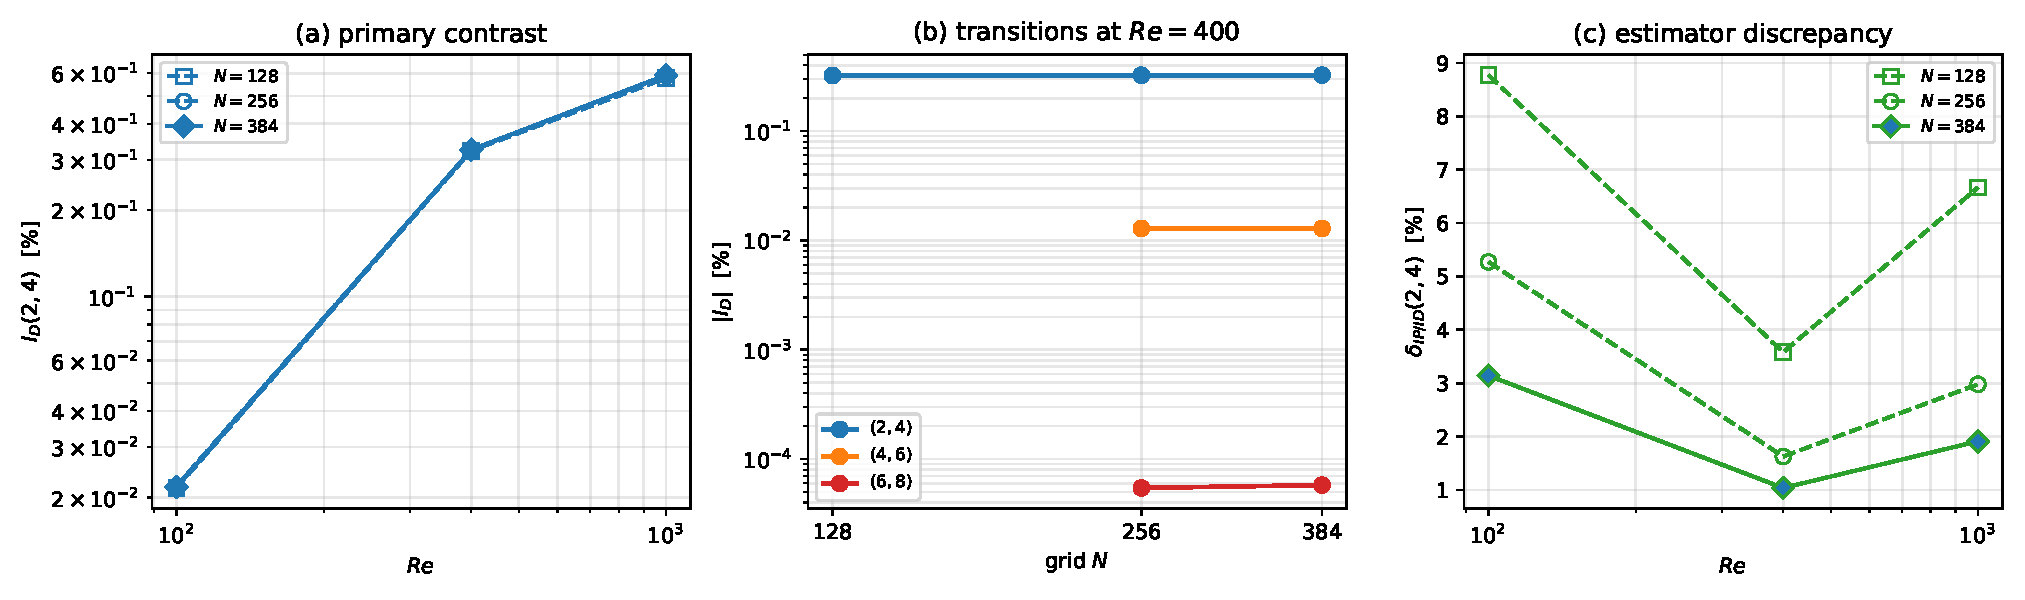
\includegraphics[width=0.85\columnwidth]{figures/figS_contrasts_res.pdf}
\caption{Resolution dependence at $\alpha=0$, with $N=384$ included in every series (open markers). (a) Primary contrast $I_D(2,4)$ for $Re=100$, $400$, $1000$. (b) All three successive transitions at $Re=400$ and $Re=1000$, the two Reynolds numbers for which $(4,6)$ and $(6,8)$ were computed; logarithmic ordinate. (c) Estimator discrepancy $\delta_{IP/ID}(2,4)$ for the three Reynolds numbers. No series contains missing or extrapolated $N=384$ points.}
\label{suppfig:contrasts_res}
\end{figure}

\subsection{Spatial decomposition of the geometric contrast}

The global contrast between $n=4$ and $n=2$ is localized exactly by partitioning the $n=4$ fluid region into the part $A$ common to both geometries and the part $B$ added by flattening. Writing $\ell$ for the local dissipation density times the cell area, the identity
\begin{equation}
\Delta D=D^*(4,0)-D^*(2,0)=\underbrace{\sum_{A}(\ell_4-\ell_2)}_{\mathrm{d}A}+\underbrace{\sum_{B}\ell_4}_{\mathrm{d}B}
\end{equation}
holds cell by cell, because $A$ and $B$ are disjoint and their union is the whole $n=4$ region. The two terms and their sum are listed in Table~\ref{supptab:layers}; the sum $\mathrm{d}A+\mathrm{d}B$ reproduces the headline contrast $I_D(2,4)$ to machine precision, and the four bands of the common region (lid, bottom, side/corner, interior core) are disjoint and sum to $\mathrm{d}A$ exactly. The interior core is negative at all three $Re$; the lid and bottom bands are positive for $Re\ge400$ and weakly negative at $Re=100$, where the largest common-region contribution is the side/corner band. The added-region term $\mathrm{d}B$ is positive at all $Re$ and grows monotonically. The redistribution term $\mathrm{d}A$ is negative only at $Re=100$ and crosses zero near $Re\approx145$ (Table~\ref{supptab:dadb}), so the net contrast $I_D(2,4)$ is positive at all Reynolds numbers while only $\mathrm{d}A$ changes sign.

\paragraph{Choice of band thresholds.}
The four-band decomposition of the common region $A$ uses thresholds chosen to isolate the physically distinct zones where dissipation concentrates or where the geometric change has its strongest effect. The \emph{lid band} (top $10\%$ of the cavity, $y>0.9$) captures the shear layer driven by the moving lid, which contains $74$--$84\%$ of the total dissipation depending on $Re$ (Section~IV.C of the main text). The \emph{bottom band} (below $y_b+0.1$, where $y_b(x)$ is the bottom-wall height) isolates the near-wall region directly affected by the superelliptic shaping; at $0.1$ in wall distance it extends just far enough above the bottom to capture the wall-normal dissipation gradient without overlapping the core. The \emph{side/corner zone} (within $0.1$ of any vertical wall) captures the lateral boundary layers and the rounded-corner fillets where the Bouzidi treatment resolves the curved geometry. The \emph{interior core} is the remainder: the bulk recirculation zone away from all walls. These thresholds ($10\%$, $0.1$) are not tuned to fit a particular result; they are round numbers of order $10\%$ that separate the cavity into its natural flow regions. A sensitivity test at $Re=400$ with alternative thresholds ($8\%$ and $12\%$ for the lid band, $0.08$ and $0.12$ for the bottom/side zones) changes the individual band contributions by at most $15\%$ but leaves the sum $\mathrm{d}A$ unchanged to machine precision (by construction, since the bands are disjoint and exhaustive) and the total contrast $I_D(2,4)$ identical. The physical interpretation---lid-dominated dissipation with a weakly dissipative added region---is therefore robust to the exact threshold values, which serve only to organize the accounting, not to determine it.

\begin{table}[!htbp]
\centering
\caption{Exact partition of the dissipation contrast $(n{=}4)-(n{=}2)$, $\alpha=0$, at $N=384$. All entries are in units of $10^{-4}D^*(2,0)$. The four bands of the common region $A$ are disjoint and sum to $\mathrm{d}A$; the added region $B$ gives $\mathrm{d}B$; their sum is $\Delta D$ and equals the headline contrast $I_D(2,4)$. Lid band: top $10\%$; bottom band: below $y_b+0.1$; side/corner: within $0.1$ of a vertical wall; core: the remainder.}
\label{supptab:layers}
\begin{tabular}{@{}lccc@{}}
\hline
Region & $Re=100$ & $Re=400$ & $Re=1000$ \\
\hline
Lid band (top $10\%$)         & $-1.33$ & $+24.42$ & $+55.51$ \\
Bottom band (below $y_b{+}0.1$)& $-1.29$ & $+6.21$ & $+23.07$ \\
Side/corner zone              & $+7.13$ & $+10.44$ & $-2.17$ \\
Interior core                 & $-9.33$ & $-28.29$ & $-65.97$ \\
\hline
$\mathrm{d}A$ (sum of bands)  & $-4.81$ & $+12.78$ & $+10.44$ \\
$\mathrm{d}B$ (added region)  & $+6.99$ & $+19.71$ & $+48.65$ \\
\hline
$\Delta D=\mathrm{d}A+\mathrm{d}B$ & $+2.18$ & $+32.49$ & $+59.09$ \\
$I_D(2,4)$ [\%]               & $+0.0218$ & $+0.3249$ & $+0.5909$ \\
\hline
\end{tabular}
\end{table}

Table~\ref{supptab:dadb} follows $\mathrm{d}A$ and $\mathrm{d}B$ along the $N=128$ Reynolds sweep. The added-region term $\mathrm{d}B$ increases monotonically throughout, whereas $\mathrm{d}A$ is negative at $Re=100$, crosses zero between $Re=100$ and $Re=150$, reaches a maximum near $Re=600$, and then decreases slowly. The two terms therefore have genuinely different Reynolds dependence, which is what makes the contrast non-power-law: $\mathrm{d}B$ grows roughly linearly in $Re$ while $\mathrm{d}A$ saturates and turns over.

\begin{table}[!htbp]
\centering
\caption{Partition $\mathrm{d}A$, $\mathrm{d}B$ and their sum along the $N=128$ Reynolds sweep, $\alpha=0$, in units of $10^{-4}D^*(2,0)$. The redistribution $\mathrm{d}A$ changes sign near $Re\approx145$.}
\label{supptab:dadb}
\begin{tabular}{@{}r|rrr@{\hskip 18pt}r|rrr@{}}
\hline
$Re$ & $\mathrm{d}A$ & $\mathrm{d}B$ & $\Delta D$ & $Re$ & $\mathrm{d}A$ & $\mathrm{d}B$ & $\Delta D$ \\
\hline
100 & $-4.73$ & $+6.89$ & $+2.16$ & 600 & $+15.62$ & $+28.21$ & $+43.83$ \\
150 & $+0.74$ & $+7.76$ & $+8.50$ & 650 & $+15.56$ & $+30.51$ & $+46.08$ \\
200 & $+4.91$ & $+9.37$ & $+14.28$ & 700 & $+15.39$ & $+32.74$ & $+48.14$ \\
250 & $+8.16$ & $+11.37$ & $+19.53$ & 750 & $+15.13$ & $+34.91$ & $+50.04$ \\
300 & $+10.63$ & $+13.63$ & $+24.26$ & 800 & $+14.80$ & $+37.00$ & $+51.80$ \\
350 & $+12.46$ & $+16.02$ & $+28.48$ & 850 & $+14.41$ & $+39.03$ & $+53.44$ \\
400 & $+13.76$ & $+18.49$ & $+32.25$ & 900 & $+13.98$ & $+40.99$ & $+54.97$ \\
450 & $+14.65$ & $+20.97$ & $+35.62$ & 950 & $+13.52$ & $+42.89$ & $+56.41$ \\
500 & $+15.21$ & $+23.43$ & $+38.64$ & 1000 & $+13.03$ & $+44.73$ & $+57.76$ \\
550 & $+15.51$ & $+25.85$ & $+41.36$ & & & & \\
\hline
\end{tabular}
\end{table}

\begin{table}[!htbp]
\centering
\caption{Grid robustness of the spatial partition $\mathrm{d}A/\mathrm{d}B$ for the primary contrast $(2,4)$ at $\alpha=0$, in units of $10^{-4}D^*(2,0)$. The four bands of the common region $A$ (lid, bottom, side/corner, core) are disjoint and sum to $\mathrm{d}A$; the added region $B$ gives $\mathrm{d}B$; their sum is $\Delta D = \mathrm{d}A + \mathrm{d}B$ and equals the headline contrast $I_D(2,4)$. Every resolution is evaluated cell by cell with the \emph{same} exact method; the $N=384$ rows reproduce Table~\ref{supptab:layers} to machine precision, so no interpolation or change of estimator is involved. The cancellation index $C=\sum|\text{bands}|/|\mathrm{d}A|$ measures the degree of internal cancellation within $\mathrm{d}A$. $N=512$ was not run at $Re=100$. The sign and order of magnitude of $\mathrm{d}A$ and $\mathrm{d}B$ are stable across all grids; the individual band magnitudes carry a grid sensitivity of up to $\sim 27\%$ at $Re=1000$, which largely cancels in $\Delta D$, whose uncertainty remains $\leq2.4\%$ of its value.}
\label{supptab:dadb_multires}
\footnotesize
\begin{tabular}{@{}cc|cccc|cccc@{}}
\hline
$Re$ & $N$ & lid & bottom & side & core & $\mathrm{d}A$ & $\mathrm{d}B$ & $\Delta D$ & $C$ \\
\hline
$100$  & $128$ & $-1.47$ & $-1.16$ & $+7.12$ & $-9.23$ & $-4.73$  & $+6.89$  & $+2.16$  & $4.0$ \\
       & $256$ & $-1.44$ & $-1.28$ & $+7.01$ & $-9.11$ & $-4.82$ & $+7.01$ & $+2.19$ & $3.9$ \\
       & $384$ & $-1.33$ & $-1.29$ & $+7.13$ & $-9.33$ & $-4.81$ & $+6.99$ & $+2.18$ & $4.0$ \\
\hline
$400$  & $128$ & $+24.48$ & $+6.55$ & $+10.22$ & $-27.48$ & $+13.76$ & $+18.49$ & $+32.25$ & $5.0$ \\
       & $256$ & $+24.36$ & $+6.18$ & $+10.27$ & $-27.88$ & $+12.91$ & $+19.55$ & $+32.46$ & $5.3$ \\
       & $384$ & $+24.42$ & $+6.21$ & $+10.44$ & $-28.29$ & $+12.78$ & $+19.71$ & $+32.49$ & $5.4$ \\
       & $512$ & $+24.34$ & $+6.18$ & $+10.41$ & $-28.23$ & $+12.71$ & $+19.78$ & $+32.49$ & $5.4$ \\
\hline
$1000$ & $128$ & $+55.90$ & $+23.92$ & $-2.61$ & $-64.19$ & $+13.03$ & $+44.73$ & $+57.76$ & $11.3$ \\
       & $256$ & $+55.43$ & $+22.84$ & $-2.53$ & $-64.99$ & $+10.75$ & $+48.02$ & $+58.77$ & $13.6$ \\
       & $384$ & $+55.51$ & $+23.07$ & $-2.17$ & $-65.97$ & $+10.44$ & $+48.65$ & $+59.09$ & $14.1$ \\
       & $512$ & $+55.39$ & $+23.05$ & $-2.26$ & $-65.96$ & $+10.22$ & $+48.95$ & $+59.18$ & $14.3$ \\
\hline
\end{tabular}
\end{table}

\begin{figure}[!htbp]
\centering
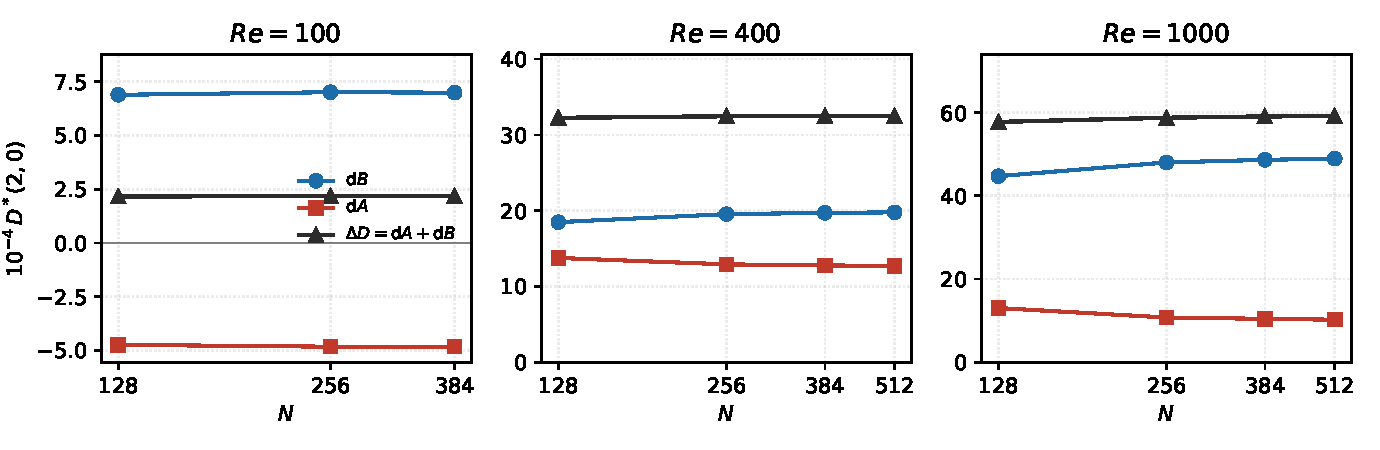
\includegraphics[width=0.98\columnwidth]{figures/figS_dadb_res.pdf}
\caption{Resolution dependence of the exact $\mathrm{d}A/\mathrm{d}B$ partition of the $(2,4)$ contrast at $\alpha=0$, in units of $10^{-4}D^*(2,0)$, computed cell by cell with the same method on each grid. The added-region term $\mathrm{d}B$ (circles) and the common-region redistribution $\mathrm{d}A$ (squares) are individually grid-sensitive --- $\mathrm{d}A$ varies by up to $\sim27\%$ at $Re=1000$ --- but their sum $\Delta D=\mathrm{d}A+\mathrm{d}B$ (triangles), which equals $I_D(2,4)$, is stable to within $2.4\%$ across all grids. $N=512$ was not run at $Re=100$.}
\label{suppfig:dadb_res}
\end{figure}

All entries in Table~\ref{supptab:dadb_multires} are recomputed from the stored velocity fields with the identical exact-partition code, so the $N=384$ rows reproduce Table~\ref{supptab:layers} to machine precision and the four bands are now available at \emph{every} resolution, including $N=128$ (which an earlier partial computation had left incomplete). The cancellation index $C$ increases both with $Re$ and, at fixed $Re$, with refinement: $4.0$ ($Re=100$), $5.0\to5.4$ ($Re=400$), and $11.3\to14.3$ ($Re=1000$) from $N=128$ to $N=512$, reflecting the growing internal cancellation within $\mathrm{d}A$ as the lid and core bands become larger and more opposed. Despite this, the net contrast $\Delta D = \mathrm{d}A + \mathrm{d}B$ --- and therefore $I_D(2,4)$ --- remains stable to within $2.4\%$ of its value across $N=128$--$512$ at all three Reynolds numbers, because the grid-induced changes in $\mathrm{d}A$ and $\mathrm{d}B$ partially cancel (Fig.~\ref{suppfig:dadb_res}).

\paragraph{Two-level interpretation of the mechanism.}
The $\mathrm{d}A/\mathrm{d}B$ decomposition supports two levels of conclusion, with different robustness to grid resolution:

\emph{Robust (qualitative) level:} (i)~The sign of $\mathrm{d}B$ is positive at all $Re$ and all $N$, confirming that the newly opened shoulder region always adds dissipation. (ii)~The sign of $\mathrm{d}A$ is negative at $Re=100$ and positive at $Re\geq 400$, confirming that the common-region redistribution changes sign near $Re\approx 145$. (iii)~The magnitude of $\mathrm{d}B$ is comparable to or larger than $\Delta D$, confirming that the sub-extensive response arises from a near-cancellation between $\mathrm{d}A$ and $\mathrm{d}B$. (iv)~The dissipation is concentrated in the lid band at $Re\geq 400$, where it accounts for $74$--$84\%$ of the total.

\emph{Quantitative level:} The individual magnitudes of the four bands and of $\mathrm{d}A$ carry a grid sensitivity that grows with $Re$: $\mathrm{d}A$ spans $0.09$ units ($1.9\%$ of itself) at $Re=100$, $1.05$ units ($8.2\%$) at $Re=400$, and $2.81$ units ($27\%$) at $Re=1000$ across $N=128$--$512$. This is the price of the internal cancellation, quantified by the rising index $C$. The sensitivity does not contaminate the net contrast $\Delta D$, whose grid dependence is bounded by $2.4\%$ across $N=128$--$512$. The quantitative mechanism---the exact balance between lid-band gain and core-band loss---is therefore best resolved at the finer grids ($N\ge256$, where the band values have settled to within a few percent), while the coarse $N=128$ bands should be read as order-of-magnitude estimates rather than converged values.

\paragraph{Alternative two-zone decomposition.}
To test whether the four-band split is essential to the conclusion, we define an alternative \emph{near-wall} zone (lid $+$ bottom $+$ side bands) and \emph{bulk} zone (core band). At $Re=400$, $N=384$, this gives $\mathrm{d}A_{\text{near-wall}} = +41.07$ and $\mathrm{d}A_{\text{bulk}} =-28.29$, with $C_{\text{alt}} = (41.07 + 28.29)/12.78 = 5.4$ (identical to the four-band $C$ by construction, since the bands are merely regrouped). The net $\mathrm{d}A = +12.78$ is unchanged. At $Re=1000$, $\mathrm{d}A_{\text{near-wall}} = +76.41$ and $\mathrm{d}A_{\text{bulk}} = -65.97$, giving $\mathrm{d}A = +10.44$ and $C_{\text{alt}} = 14.1$. The qualitative conclusion---that $\mathrm{d}A$ is a near-cancellation between opposing near-wall and bulk contributions---is therefore independent of the four-band split; the split serves only to localize the cancellation within the near-wall region (between lid, bottom, and side) and the bulk (core).

\begin{figure}[!htbp]
\centering
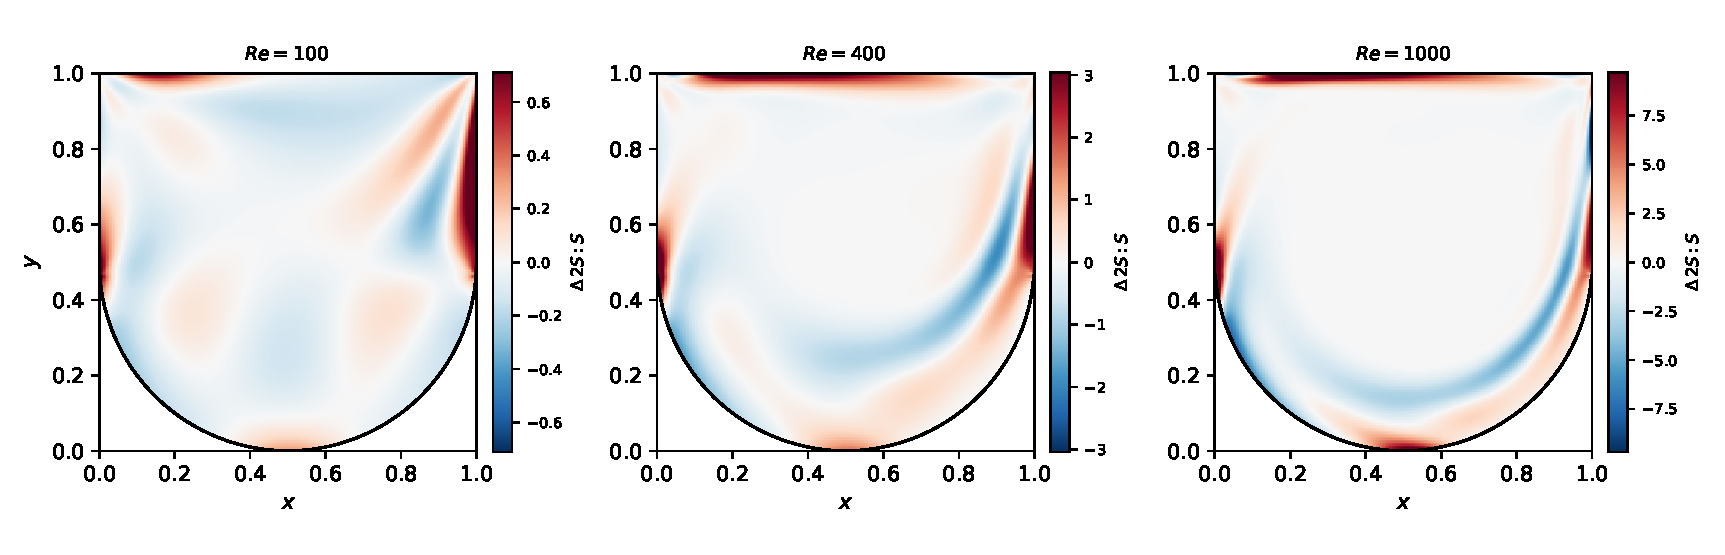
\includegraphics[width=0.98\columnwidth]{figures/figS_deltaD_maps.pdf}
\caption{Local dissipation contrast $\Delta(2\mu\mathbf{S}{:}\mathbf{S})=(n{=}4)-(n{=}2)$ at $\alpha=0$, $N=384$, evaluated on the $n=2$ region, for $Re=100$, $400$, $1000$. The lid and bottom bands are positive at $Re\ge400$ and weakly negative at $Re=100$, the interior core is negative throughout, and the net contrast $I_D(2,4)$ remains positive at all three Reynolds numbers.}
\label{suppfig:deltaD}
\end{figure}

\subsection{Reynolds-number sweep}

The exploratory parameter sweep at $N=128$, with complete LBM parameters recorded in Table~\ref{supptab:resweep_params}, resolves the continuous variation of the primary contrast $I_D(2,4)$ at $\alpha=0$ (Table~\ref{supptab:resweep}). The local logarithmic slope $\gamma_{\rm loc}=d\ln|I_D|/d\ln Re$ decreases monotonically from $2.72$ near $Re=150$ to $0.47$ near $Re=950$ (the central-difference estimate ends one interval before the largest $Re$), crossing unity near $Re\approx346$. As discussed in the main text, this smooth inflection reflects the competition between the linear growth of the added-region dissipation and the saturation of common-region redistribution; the value $Re\approx346$ is reported as a descriptive feature of this coarse-grid trajectory, not an exact universal scaling law.

\begin{table}[!htbp]
\centering
\caption{Primary contrast $I_D(2,4)$ at $\alpha=0$ from the $N=128$ exploratory Reynolds sweep.}
\label{supptab:resweep}
\begin{tabular}{@{}cc|cc@{}}
\hline
$Re$ & $I_D$ [\%] & $Re$ & $I_D$ [\%] \\
\hline
100 & 0.02160 & 150 & 0.08500\\
200 & 0.14280 & 250 & 0.19534\\
300 & 0.24259 & 350 & 0.28482\\
400 & 0.32251 & 450 & 0.35619\\
500 & 0.38640 & 550 & 0.41363\\
600 & 0.43829 & 650 & 0.46078\\
700 & 0.48139 & 750 & 0.50038\\
800 & 0.51798 & 850 & 0.53437\\
900 & 0.54968 & 950 & 0.56405\\
1000 & 0.57758 & \\
\hline
\end{tabular}
\end{table}

\subsection{Robustness tests}

\emph{Wall-gradient treatment.} Replacing the geometric wall-distance correction of the bottom-wall one-sided gradient by a purely node-based one-sided difference changes $I_D(2,4)$ from $0.0218\%$ to $0.0207\%$ ($Re=100$), $0.3249\%$ to $0.3212\%$ ($Re=400$), and $0.5909\%$ to $0.5777\%$ ($Re=1000$); the contrast changes by $5.0\%$ of its own value at $Re=100$ and by only $1.1$--$2.2\%$ at $Re=400$--$1000$.

\emph{Effective-Reynolds perturbation.} A $0.4\%$ differential shift of the effective Reynolds number between the two geometries propagates to a change of $0.0005\%$ in $I_D(2,4)$ at $Re=100$ ($2\%$ of its value) and $0.0011\%$ at $Re=400$ ($0.4\%$).

\emph{Grid span.} Because the residual change between the two finest grids is dominated by the partial cancellation of common discretization error rather than by a clean power-law decay, no Richardson extrapolation or GCI is quoted; the span of $I_D(2,4)$ over $N=128$--$384$ is taken as the conservative numerical uncertainty: $3.4\times10^{-4}$ percentage points ($Re=100$), $2.4\times10^{-3}$ ($Re=400$), $1.3\times10^{-2}$ ($Re=1000$), i.e.\ at most $2.3\%$ of the finest-grid contrast.

\emph{Discrete versus analytic area.} The discrete fluid area differs from the analytic value of \texttt{area\_fluid} by at most $0.017\%$ over all cases, so the choice of discrete or analytic reference area does not affect any quoted contrast.

\section{Area-based reference model and supplementary analyses}
\label{suppsec:area}

\subsection{Area reference model}

The area-only reference assumes that the change in dissipation across a geometric transition is explained solely by the change in fluid area:
\begin{equation}
I_{D,\mathrm{area}}(q_i,q_j) = \frac{A_f(q_j)-A_f(q_i)}{A_f(q_i)}\times 100\%.
\end{equation}
The fluid area is not constant across the exponent transitions: it grows from $A_f=0.8927$ ($n=2$) to $0.9635$ ($n=4$), $0.9819$ ($n=6$), and $0.9892$ ($n=8$) at $\alpha=0$. Here $A_f^{\rm analytic}=HL-\int y_b\,dx$ is the exact analytic superellipse area; the discrete mask area recorded in the numerical outputs, $A_f^{\rm mask}$, differs from it by at most $\sim0.02\%$ at $N=384$ (e.g.\ $0.96356$ versus $0.963519$ for $n=4$). The reference model uses the analytic area, while the saved scalars report the mask area; the two agree to well within the resolution uncertainty quoted throughout. The model therefore predicts nonzero positive contrasts, $+7.93\%$, $+1.91\%$, and $+0.75\%$ for $(2,4)$, $(4,6)$, and $(6,8)$, respectively. Table~\ref{supptab:area} compares these predictions with the measured values. The measured contrasts are smaller than the prediction by factors ranging from $13$ (the $(2,4)$ transition at $Re=1000$, where the geometric response is strongest) to $1.3\times10^{4}$ (the $(6,8)$ transition at $Re=400$, where the trailing contrast nearly vanishes). They share the sign of the prediction for every transition at $Re=100$ and $Re=400$ and for $(4,6)$ at $Re=1000$, but not for $(6,8)$ at $Re=1000$, where the measured contrast is resolved and negative: the extensive area reference cannot produce a negative contrast, so this is the clearest single indication that the area-only model is a scale reference rather than a prediction. Two entries of the table are flagged as upper bounds, for the reasons given in Section~\ref{suppsec:contrasts}: the $Re=100$ $(4,6)$ contrast cannot be resolution-tested at that Reynolds number, and the $Re=400$ $(6,8)$ contrast falls inside its own $N=128$--$384$ span. The area-only model is therefore a simple extensive reference, not a quantitative prediction of the energetic response.

\begin{table}[!htbp]
\centering
\caption{Comparison with the area-based reference model at $N=384$, $\alpha=0$. The measured contrast $I_D$ is compared with the area-only prediction $I_{D,\mathrm{area}}$; the ratio is given in absolute value, and the sign of the measured contrast is stated explicitly where it differs from the prediction.}
\label{supptab:area}
\begin{tabular}{@{}ccccc@{}}
\hline
Transition & $Re$ & $I_D$ [\%] & $I_{D,\mathrm{area}}$ [\%] & ratio \\
\hline
$(2,4)$ & $100$  & $+0.0218$ & $+7.93$ & $364$ \\
$(2,4)$ & $400$  & $+0.3249$ & $+7.93$ & $24.4$ \\
$(2,4)$ & $1000$ & $+0.5909$ & $+7.93$ & $13.4$ \\
$(4,6)$ & $100$  & $+0.00296$& $+1.91$ & $645$ (upper bound) \\
$(4,6)$ & $400$  & $+0.0129$ & $+1.91$ & $148$ \\
$(4,6)$ & $1000$ & $+0.0103$ & $+1.91$ & $185$ \\
$(6,8)$ & $100$  & $+0.00042$& $+0.75$ & $1786$ \\
$(6,8)$ & $400$  & $+0.00006$& $+0.75$ & $1.3\times10^{4}$ (upper bound) \\
$(6,8)$ & $1000$ & $-0.0037$ & $+0.75$ & $203$ (sign reversed) \\
\hline
\end{tabular}
\end{table}

\subsection{Amplitude interaction}

When both amplitude values $\alpha=0$ and $\alpha=0.1$ are available for the same $(Re,n)$ pair, the effect of $\alpha$ is a downward shift of $P^*$ and $D^*$ consistent with the reduction of the fluid area from $A_f=0.8927$ ($\alpha=0$) to $A_f=0.8427$ ($\alpha=0.1$) at $n=2$. More importantly, the amplitude modifies the magnitude of the geometric contrast itself. At $Re=400$ the $(2,4)$ dissipation contrast is $+0.3249\%$ at $\alpha=0$ and $+0.1333\%$ at $\alpha=0.1$; at $Re=1000$ it is $+0.5909\%$ and $+0.0782\%$; at $Re=100$ it is $+0.0218\%$ and $+0.0081\%$. The hierarchy of the contrasts across $n$ is preserved at both amplitudes, but its quantitative strength is weaker when the wall is undulated. The trailing transitions change sign with amplitude at $Re\ge400$: at $Re=400$ the $(4,6)$ and $(6,8)$ contrasts are $+0.0129\%$ and $+0.00006\%$ at $\alpha=0$ but $-0.0039\%$ and $-0.0017\%$ at $\alpha=0.1$, and at $Re=1000$ they are $+0.0103\%$ and $-0.0037\%$ at $\alpha=0$ and $-0.0242\%$ and $-0.0052\%$ at $\alpha=0.1$ (Table~\ref{supptab:contrasts}). At $Re=100$, by contrast, both trailing contrasts stay positive under undulation but weaken further, from $+0.00296\%$ to $+0.00098\%$ for $(4,6)$ and from $+0.00042\%$ to $+0.00006\%$ for $(6,8)$. At the undulated wall, therefore, increasing the exponent beyond $n=4$ slightly reduces the dissipation at $Re=400$ and $Re=1000$, while at $Re=100$ it still increases it, by an amount at the resolution floor.

\begin{table}[!htbp]
\centering
\caption{Effect of the undulation amplitude on the $(2,4)$ dissipation contrast at $N=384$.}
\label{supptab:amplitude}
\begin{tabular}{@{}ccc@{}}
\hline
$Re$ & $I_D(2,4)$, $\alpha=0$ [\%] & $I_D(2,4)$, $\alpha=0.1$ [\%] \\
\hline
$100$  & $+0.0218$ & $+0.0081$ \\
$400$  & $+0.3249$ & $+0.1333$ \\
$1000$ & $+0.5909$ & $+0.0782$ \\
\hline
\end{tabular}
\end{table}

\clearpage

\section{Data and reproducibility note}
\label{suppsec:repro}

The scalar results are stored as JSON files in the directory \texttt{results/scalars/}, one file per converged simulation, and are consolidated into the table \texttt{scalars\_clean.csv} used for the figures and tables of the main text. Each JSON file contains the following fields: \texttt{Re}, \texttt{n}, \texttt{alpha}, \texttt{N}, \texttt{P\_star}, \texttt{D\_star}, \texttt{K\_star}, \texttt{fluid\_area}, \texttt{Ma}, \texttt{iters}, \texttt{residual}, \texttt{status}. The velocity fields are stored as NumPy \texttt{.npz} files in \texttt{results/fields/}, with arrays \texttt{ux}, \texttt{uy}, \texttt{rho}, \texttt{fluid} (boolean mask), and the grid coordinates \texttt{xc}, \texttt{yc}.

All figures in the main manuscript and in this supplementary material were generated from these files using Python scripts with Matplotlib. The sign conventions, normalizations, and contrast definitions used in the scripts are exactly those stated in the main manuscript (Sections~II.E and~II.G). The complete scalar dataset, converged velocity field arrays, and post-processing scripts are available from the corresponding author upon reasonable request (and will be deposited in an open-access Zenodo repository upon publication).

\begin{table}[!htbp]
\centering
\caption{Energy-balance defect $\varepsilon_E = |P^*-D^*|/D^* \times 100\%$ for $n=2$ and $n=4$ at $\alpha=0$, and the primary contrast $I_D(2,4)$, versus grid resolution $N$ at $Re=100$ and $Re=400$. The defect decreases by approximately a factor of 3 between $N=128$ and $N=384$ (from $\sim5.8\%$ to $\sim2.0\%$ at $Re=100$, and from $\sim6.2\%$ to $\sim2.0\%$ at $Re=400$), while the contrast $I_D(2,4)$ remains stable to within $3.4\times10^{-4}$~pp ($1.6\%$ of its value) at $Re=100$ and $2.4\times10^{-3}$~pp ($0.7\%$) at $Re=400$. This demonstrates that the absolute defect is a common-mode error that cancels in the paired contrast $\Delta D = D^*(4)-D^*(2)$, whose grid sensitivity is an order of magnitude smaller than that of the defect itself.}
\label{supptab:defect_vs_contrast}
\begin{tabular}{@{}c|c|cc|cc@{}}
\hline
$Re$ & $N$ & $\varepsilon_E(n{=}2)$ [\%] & $\varepsilon_E(n{=}4)$ [\%] & $\Delta\varepsilon$ [\%] & $I_D(2,4)$ [\%] \\
\hline
$100$ & $128$ & $5.790$ & $5.793$ & $0.003$ & $0.02161$ \\
      & $256$ & $2.766$ & $2.770$ & $0.004$ & $0.02195$ \\
      & $384$ & $1.976$ & $1.977$ & $0.001$ & $0.02178$ \\
\hline
$400$ & $128$ & $6.204$ & $6.193$ & $0.011$ & $0.32251$ \\
      & $256$ & $3.199$ & $3.194$ & $0.005$ & $0.32462$ \\
      & $384$ & $2.041$ & $2.038$ & $0.003$ & $0.32488$ \\
\hline
\end{tabular}
\end{table}

The variation of the defect between $N=128$ and $N=384$ is $\Delta\varepsilon_E \approx 3.4$ percentage points at $Re=100$ and $\approx 4.2$ points at $Re=400$, while the contrast $I_D(2,4)$ varies by only $3.4\times10^{-4}$~pp and $2.4\times10^{-3}$~pp, respectively---i.e., four to five orders of magnitude less. The defect is therefore a common-mode resolution error of the absolute integrals $P^*$ and $D^*$ that cancels in their paired difference. The small residual $\Delta\varepsilon_E$ between $n=2$ and $n=4$ at fixed $N$ (third column) is at most $0.011\%$, which bounds the contamination of the contrast by differential defect effects to well below the quoted span.


\bibliography{references}

\end{document}
